%\documentclass[11pt,a4paper]{article}
%\documentclass[11pt,a4paper]{scrartcl}
\documentclass[11pt,a4paper,oneside]{book}
\usepackage[table]{xcolor}
\usepackage{colortbl}
\usepackage{tabularray}
\usepackage{pgfplots}
\usepackage[british,UKenglish,USenglish,english,american]{babel}
%\usepackage[a4paper, total={16cm, 23cm}]{geometry}
\usepackage[tmargin = 1.25in,bmargin = 1.25in,lmargin = 1in,rmargin = 1in]{geometry}
\usepackage{tikz}
\usepackage{graphicx}
\usepackage[version=4]{mhchem}
\usepackage{chemformula}

\usepackage{enumitem}
\usepackage{makeidx}
\usepackage{epstopdf}
\usepackage{amssymb}
\usepackage{mathrsfs}
\usepackage{amsmath}

\usepackage[english]{varioref}
\usepackage[english]{babel}
\usepackage{lipsum}
\usepackage{fancyhdr}
\pagestyle{fancy} 
\usepackage{float}
\usepackage{empheq}
\usepackage[framemethod=tikz]{mdframed}
\usepackage{epstopdf}
\numberwithin{equation}{section}
\usepackage{eso-pic}
\usepackage{calc}
\usepackage{nccmath}
\usepackage{caption}
\usepackage{subcaption}
\usepackage{gensymb}
\usepackage{amsfonts,amsthm,epsfig,epstopdf,titling,url,array}
\usepackage{siunitx}
\usepackage{xcolor}
\usepackage{multicol}
\usepackage{boondox-cal}
\usepackage{tabularray}


\setcounter{secnumdepth}{3}
\setcounter{tocdepth}{3}
\usepackage{booktabs}

\DeclareSIUnit\atm{atm}

\pagestyle{fancy} 
\fancypagestyle{firstpage}{}
\fancyhead[L]{\slshape\nouppercase{\leftmark}}
\chead{}
\rhead{}
\lfoot{\textit{}}
\cfoot{-\ \thepage\ -}
\rfoot{\textit{}}

\DeclareMathOperator{\rank}{rank}
\DeclareMathOperator{\atantwo}{atan2}

\renewcommand{\headrulewidth}{0.4pt}
\renewcommand{\footrulewidth}{0.4pt}
\newcommand{\abs}[1]{\left|#1\right|}
\definecolor{mycolor1}{rgb}{0.95, 0.95, 0.95}
\definecolor{mycolor2}{rgb}{0.95, 0.95, 0.95}
\definecolor{tableShade}{gray}{0.9}
\newcommand{\sign}{\text{sign}}
\newcommand{\centered}[1]{\begin{tabular}{@{}l@{}} #1 \end{tabular}}
\theoremstyle{it}
\newtheorem{defn}{Definition}[section]
\newtheorem{thm}{Theorem}[section]
\newtheorem{lemma}{Lemma}[section]
\theoremstyle{definition}
%\theoremstyle{it}
\newtheorem{example}{Example}[section]

\newenvironment{myitemize_1}
{ \begin{itemize}[topsep=0pt]
		\setlength{\topsep}{2pt}		
		\setlength{\itemsep}{2pt}
		\setlength{\parskip}{2pt}
		\setlength{\parsep}{2pt}     }
	{ \end{itemize}                  }


\newmdenv[innerlinewidth=0.5pt, roundcorner=4pt,backgroundcolor=mycolor2, linecolor=mycolor1,innerleftmargin=6pt,
innerrightmargin=6pt,innertopmargin=6pt,innerbottommargin=6pt]{mybox}

\title{\textbf{Electrification of Heavy Duty Vehicles}}
\author{Davide Bagnara}

\begin{document}
	\thispagestyle{firstpage}
	\begin{mybox}
  		\maketitle
		\vspace{125mm}
	\end{mybox}
	\newpage
	\tableofcontents
	\listoffigures	
	\listoftables
	\newpage

\chapter{Introduction}
\section{Scope of the project}
Scope of the project is to design an electrical power-train of a heavy duty vehicle, in particular of a bulldozer tracked vehicle. The original power-train configuration is made by a diesel engine (power source) followed by two hydrostatic transmissions (one for each track), which each one is made by a hydraulic pump and a hydraulic motor.  The mechanical end of each hydrostatic transmission is connected to a driver gear which, in turn, is connected to the track of the vehicle. The electrification consists of designing all the components which are necessary in order to replace the whole functionalities of the original vehicle. In order to identify the main components necessary for the design of an electrical vehicle it is necessary to consider to different case study
\begin{itemize}
	\item[--] Full electrification: the whole system consisting of diesel engine and hydrostatic transmission is replaced by an electrical drive train. 
	\item[--] Power source electrification: the only diesel engine and the source of power is electrified. The internal hydrostatic transmission is not modified.
\end{itemize}
The main components which can be preliminary identified are as follows
\begin{itemize}
	\item[--] A power source 
		\begin{itemize}
			\item[--] PEM fuel cell (optional) 
			\item[--] Battery accumulator like lithium-ion battery	
		\end{itemize}
	\item[--] An electrical drives based on inverter 
	\item[--] An electrical motor which in general, due to torque weight ratio, is a permanent magnet synchronous machine (PMSM).
\end{itemize} 
Additional components are 
\begin{itemize}
	\item[--] A DC/DC converter, mandatory in the case of PEM fuel cell
	\item[--] A bidirectional DC/DC converter with insulation (optional) for ancillary service
\end{itemize}

Concerning the power source, in this project, the use of a PEM fuel-cell is taken into account.

The operative part of the project consists into the modelization, via \textbf{simscape} - Matlab/Simulink environment, of the main components and in the implementation of the whole control strategy. In such a way, the output of the project is a set of mathematical models and a collection of the main design criteria which have been encountered during the design of the electrification. 

The following document, will trace a guideline path concerning the design of the electrification. 

\section{Structure of the document}
The document contains three parts
\begin{itemize}
	\item[--] \textbf{The hydrostatic power-train} -- here the description of the actual heavy duty vehicle is reported. Additional information regarding the vehicle control are also reported.
	\item[--] \textbf{Electrification of the hydrostatic power-train} -- here a more in deep description of the main electrical equipments are reported.
	\item[--] \textbf{Case study} -- here some case study of electrification are reported.
\end{itemize}


\part{Hydrostatic Power-train}
\chapter{Hydrostatic transmission}
\section{Dynamical Mathematical model}
The heavy duty vehicle power-train is, in general, performed by a diesel engine followed by two hydrostatic transmissions (one for each truck), where each one is composed by a variable displacement hydraulic pump followed by a variable (or fixed) displacement hydraulic motor. In the following, we will consider the case where both pump and motor are equipped with a adjustable displacements (which means variable volumetric flow). 

The use of both adjustable volumetric displacement pump and motor permits to extend the operating working area, in terms of speed and torque, of the whole transmission line.  Basically, this kind of transmission is often identified as a continuous variable gear-ratio.
Figure~\ref{hydro_transm_1} depicts a typical hydrostatic power train, where the dynamic equations can be represented as follows

\vspace{5mm}
\textbf{Section \textit{R}.}
\begin{equation}\left\lbrace 
	\begin{aligned}
		\Delta \dot{p}_R &= \frac{1}{\beta}\Big[D_p^R\omega_p^R - D_m^R \omega_m^R - q_d^R \Big] \\[8pt]
		\dot{\omega}_m^R &= \frac{1}{J_m}\Big[\tau_m^R -\tau_\vartheta^R - b_m\omega_m^R \Big] \qquad\text{where} \qquad \tau_m^R = D_m^R \Delta p_R \\[8pt]
		\dot{\omega}_l^R &= \frac{1}{J_l}\Big[\tau_\vartheta^R n_m/n_l - \tau_l^R - b_l\omega_l^R \Big]\\[8pt]
		\dot{\tau}_\vartheta^R &= k_\vartheta\Big[\omega_m^R -\omega_l^R n_m/n_l\Big]
	\end{aligned}\right. 
\end{equation}
where $D_m^R = d_m^R V_m^{nom}$, $D_p^R = d_p^R V_p^{nom}$ and where $V^{nom}$ means the nominal volumetric displacement of the pump or motor.

The term $D_p\omega_p$ represents the total flow at the output of the pump, while the term $D_m\omega_m$ represents the total flow at the input of the motor. The equation $\Delta \dot{p} = \frac{1}{\beta}\Big[D_p\omega_p - D_m \omega_m - q_d \Big]$ represents the continuity's law of the hydrostatic driveline.
\begin{figure}[H]
	\centering
	\includegraphics[width = 450pt, angle = 0, keepaspectratio]{figures/hydrostatic_transmission_RL.eps}
	\captionsetup{width=0.5\textwidth, font=small}		
	\caption{Hydrostatic transmission - the whole transmission power-train is made two, independent lines, one for the left side (\textit{L}) and one for the right side (\textit{R}) as follows.}
	\label{hydro_transm_1}
\end{figure}
\textbf{Section \textit{L}.}
\begin{equation}\left\lbrace 
	\begin{aligned}
		\Delta \dot{p}_L &= \frac{1}{\beta}\Big[D_p^L\omega_p^L - D_m^L \omega_m^L - q_d^L \Big] \\[8pt]
		\dot{\omega}_m^L &= \frac{1}{J_m}\Big[\tau_m^L - \tau_\vartheta^L - b_m\omega_m^L\Big] \qquad\text{where}\qquad\tau_m^L = D_m^L \Delta p_L \\[8pt]
		\dot{\omega}_l^L &= \frac{1}{J_l}\Big[\tau_\vartheta^L n_m/n_l - \tau_l^L - b_l\omega_l^L \Big]\\[8pt]
		\dot{\tau}_\vartheta^L &= k_\vartheta\Big[\omega_m^L -\omega_l^L n_m/n_l\Big]
	\end{aligned}\right. 
\end{equation}
where $D_m^L = d_m^L V_m^{nom}$, $D_p^L = d_p^L V_p^{nom}$ and where $V^{nom}$ means the nominal volumetric displacement of the pump or motor.

Equations of the source side (engine) can be written as follows
\begin{equation}\left\lbrace 
	\begin{aligned}
		\dot{\omega}_e &=\frac{1}{J_e}\Big[\tau_e -\tau_{p_\vartheta}^{R}-\tau_{p_\vartheta}^{L} - b_p\omega_e\Big] \\[8pt]
		\dot{\omega}_p^R &=\frac{1}{J_p}\Big[\tau_{p_\vartheta}^{R}-\tau_p^R - b_p\omega_p^R\Big] \\[8pt]
		\dot{\omega}_p^L &=\frac{1}{J_p}\Big[\tau_{p_\vartheta}^{L}-\tau_p^L - b_p\omega_p^L\Big] \\[8pt]
		\dot{\tau}_{p_\vartheta}^{R} &= k_\vartheta \Big[ \omega_e - \omega_p^R\Big] \\[8pt]
		\dot{\tau}_{p_\vartheta}^{L} &= k_\vartheta \Big[ \omega_e - \omega_p^L\Big]
	\end{aligned}\right. 
\end{equation}
This final group of equations represent the Newton's law at the engine side.

\section{Steady state equations}
An important aspect, which has to be taken into account, is the evaluation of the hydrostatic transmission in steady state condition and the relations among torques and rotational speeds, as follows
\begin{equation}\label{steady_1}
	\begin{aligned}
		\eta_p^vD_p\omega_p=\frac{D_m\omega_m}{\eta_p^v}
	\end{aligned}
\end{equation}
Eq.~\eqref{steady_1} represent the steady state flow balance between pump and motor. The terms $\eta_p^v$ and $\eta_m^v$ are the volumetric efficiency of the pump and motor respectively. Eq.~\eqref{steady_1} can be also represented as follows
\begin{equation}\label{steady_2}
	\boxed{	\begin{aligned}
			\omega_m=\Bigg(\frac{D_p}{D_m}\Bigg)\omega_p\Big(\eta_p^v\eta_m^v\Big)
	\end{aligned}}
\end{equation}
where eq.~\eqref{steady_2} shows that the hydraulic motor speed is proportional to the pump volumetric displacement and inversely proportional to the motor volumetric displacement.

The equation Eq.~\eqref{steady_3} represents a balance of power among pump and motor 
\begin{equation}\label{steady_3}
	\begin{aligned}
		\frac{\tau_m\omega_m}{\eta_m^m}=\eta_p^m\tau_p\omega_p
	\end{aligned}
\end{equation}
and can also be represented as shown in Eq.~\eqref{steady_4}
\begin{equation}\label{steady_4}
	\boxed{	\begin{aligned}
			\tau_p =\frac{1}{\eta_p^m\eta_m^m}\Bigg(\frac{D_p}{D_m}\Bigg)\tau_m
	\end{aligned}}
\end{equation}
where $\eta_p^m$ and $\eta_m^m$ are the mechanical efficiency of the pump and motor respectively, $D_m = V_m^{nom}d_m$ where $$d_m\in\big[0.36,\ 1\big] = \big[d_m^{min},\ d_m^{max}\big]$$ and $D_p = V_p^{nom}d_p$ where $$d_p\in\big[-1,\ 1\big] = \big[-d_p^{max},\ d_p^{max}\big].$$

The torque which the engine has to sustain (for steady-state condition)  is proportional to the load and to the pump volumetric displacement and inversely proportional to the motor volumetric displacement.


\chapter{Driver gear model}
The hydraulic motor is connected to the track (undercarriages) via a gear device which is also called \textit{drive-gear}, see also Figure~\ref{travel_gear}. 
\begin{figure}[H]
	\centering
	\includegraphics[width = 300pt, angle = 0, keepaspectratio]{figures/travel_gear.eps}
	\captionsetup{width=0.5\textwidth, font=small}		
	\caption{Drive-gear representation.}
	\label{travel_gear}
\end{figure}
Along this document we suppose that the rotational low speed side has been measured for condition monitoring and control.

The mathematical model of the gear is here reported in a very simplified form: 
\begin{equation}
	\omega_l=\omega_m/n_{tg}
\end{equation}
where $\omega_l$ is the low speed high torque side connected to the track and $\omega_m$ is the high speed low torque connected to the hydraulic motor. The term $n_{tg}$ represents the ratio between high speed and low speed of the gear.

The planetary gear or \textit{driver gear} is here modelled as a flexible shaft (as already reported), 
\begin{equation}\left\lbrace 
	\begin{aligned}
		\dot{\omega}_m &= \frac{1}{J_m}\Big[\tau_m - \tau_\vartheta^m - b_m\omega_m\Big] \\[8pt]
		\dot{\omega}_l &= \frac{1}{J_l}\Big[\tau_\vartheta^l - \tau_l - b_l\omega_l \Big] \\[8pt]
		\dot{\tau}_\vartheta &= k_\vartheta\Big[\omega_m -\omega_l n_{tg} \Big] \\[8pt]
		n_{tg} &= \frac{n_m}{n_l} \\[8pt]
		\tau_\vartheta &= \tau_\vartheta^m=\frac{\tau_\vartheta^l}{n_{tg}}
	\end{aligned}\right. 
\end{equation}
where $\tau_\vartheta^m$ is the torsional torque seen at high speed gear side as well as $\tau_\vartheta^l$ is the torsional torque seen at low speed gear side, see also Figure~\ref{flexshaft}.
\begin{figure}[H]
	\centering
	\includegraphics[width = 425pt, angle = 0, keepaspectratio]{figures/gear_flexshaft_1.eps}
	\captionsetup{width=0.5\textwidth, font=small}		
	\caption{Drive-gear representation as flexible shaft model.}
	\label{flexshaft}
\end{figure}


A practical example can be as follows.

Let $n_{tg}=41.4$ be the gear ratio of the \textit{drive-gear} and let $R=\SI{0.44056}{\meter}$ be its radius. Considering a maximum (nominal) vehicle speed of $v_{tr} = \SI{11}{\kilo\meter\per\hour}$ we obtain a maximum (nominal) hydraulic motor speed of $\omega_m^{nom} = \SI{2742}{\per\minute}$, see also Figure~\ref{track_1}. 
\begin{figure}[H]
	\centering
	\includegraphics[width = 200pt, angle = 0, keepaspectratio]{figures/track_1.eps}
	\captionsetup{width=0.5\textwidth, font=small}		
	\caption{Track representation.}
	\label{track_1}
\end{figure}

\chapter{Pump and motor volumetric displacement actuator}
The pump or motor swash-plate is, in general, actuated by a hydrostatic servo, which is followed by a valve and an electromechanical system actuators. The overall dynamic, which means the dynamic how the swash-plate position is actuated (that means also the dynamic how a certain amount of volumetric displacement is set), plays an important role into the dynamic response of the hydrostatic power-train. Hence, as shown in Figure~\ref{sp_actuator}, the pump and motor swash-plate actuator can be summarized by a four way spool valve, which is driven by an electromechanical actuator (solenoid or permanent magnet moving coil), and by a double chamber servo actuator. The overall plant, in term of  mathematical model (electromechanical and hydrostatic), can be linearized by a double integrator (see also Chapter~\ref{appendix_A}), as follows
\begin{equation}\label{swash_plate_actuator}
	D(s) = k\frac{1}{s^2}U(s)
\end{equation}
where $D(s)$ represents the per unit volumetric displacement $d(t)$ and $U(s)$ is the control input. 
Hence, the model represented by eq.~\eqref{swash_plate_actuator} is the transfer function between the voltage input (voltage which controls the electromechanical actuator) and the per unit volumetric displacement which is directly correlated to the actual volumetric flow which is also correlated to the position of the swash-plate.  

The control architecture of the volumetric displacement is assumed to be implemented as a state feedback control, see also Figure~\ref{sf_ctrl_displacement}.

\begin{figure}[H]
	\centering
	\includegraphics[width = 475pt, angle = 0, keepaspectratio]{figures/swashplate_actuator_2.eps}
	\captionsetup{width=0.5\textwidth, font=small}		
	\caption{Swash-plate actuator.}
	\label{sp_actuator}
\end{figure}
The whole volumetric displacement system (model and control) of both pump and motor can be modelized in state space form as follows (see also Figure~\ref{sf_ctrl_displacement}).

The transfer function $$H(s) = k\frac{1}{s^2}$$ can be represented in state space form using the controllable canonical form as follows
\begin{equation}\label{ssr1}
	\tilde{\mathbf{A}} = \begin{bmatrix}
		0 & 1 \\[6pt]
		0 & 0
	\end{bmatrix} \qquad
	\tilde{\mathbf{B}} = \begin{bmatrix} 0\\[6pt] 1\end{bmatrix} \qquad
	\mathbf{C} = \begin{bmatrix}
		k & 0
	\end{bmatrix}
\end{equation}
Resulting in the following system
\begin{equation}\label{ssr2}
	\begin{aligned}
		\dot{\vec{x}}(t) &=\tilde{\mathbf{A}} \vec{x}(t) + \tilde{\mathbf{B}} u(t) \\[6pt]
		y(t) &= \mathbf{C}\vec{x}(t)
	\end{aligned}
\end{equation}
where $y(t) = d(t)$. For more details see Chapter~\ref{appendix_A}.
\begin{figure}[H]
	\centering
	\includegraphics[width = 400pt, keepaspectratio]{figures/swashplate_model_ctrl_2.eps}
	\captionsetup{width=0.5\textwidth, font=small}		
	\caption{State feedback control of the volumetric displacement actuator.}
	\label{sf_ctrl_displacement}
\end{figure}

\chapter{Diesel engine model}
In this section the description of the IC-engine is reported. The knowledge of the torque and power curve of the engine plays an important role in the performance of the engine anti-stall control.

In the following, we describe how the IC-engine has been modelized. We start to consider two curves:
\begin{itemize}
	\item Torque curve: maximum torque available for a given rotor speed and maximum displacement of the throttle.
	\item Torque friction curve: torque generated by the friction for a given rotor speed. This friction is considered always present, for any value of the throttle. See also Figure~\ref{engine_curves}
\end{itemize}
The mechanical model of the engine can be described as follows
\begin{equation}
	J\frac{d\omega_e}{dt} = \theta_f(t)\tau^{nom}(\omega_e) + \tau^{b}(\omega_e) - \tau_{load}
\end{equation}
where $\tau^{nom}(\omega_e)$ and $\tau^{b}(\omega_e)$ are shown in Figure~\ref{engine_curves} while $\theta_f(t)$ is the throttle which is generated by the external speed loop control as shown in Figure~\ref{engine_ctrl_1} and $J=\SI{7.5}{\kilogram\per\square\meter}$.

The speed control is performed by a PI-controller and it adapts the throttle displacement in order to keep the request speed tracked.

An additional second order filter is taken into account in order to modelize additional dynamics.

The controller can be described as follows
\begin{equation}
	\left\lbrace \begin{aligned}
		&\tilde{\omega}_e(t) = \frac{1}{\omega_e^{\text{nom}}}\Big(\omega^{\text{ref}}_e - \omega_e(t)\Big)\\[6pt]
		&\theta(t) = k_p\,\tilde{\omega}_e(t) + \theta^i(t) \\[6pt]
		&\frac{d\theta^i}{dt}(t) = k_i\,\tilde{\omega}_e(t)	
	\end{aligned}\right. 
\end{equation}
\begin{figure}[H]
	\centering
	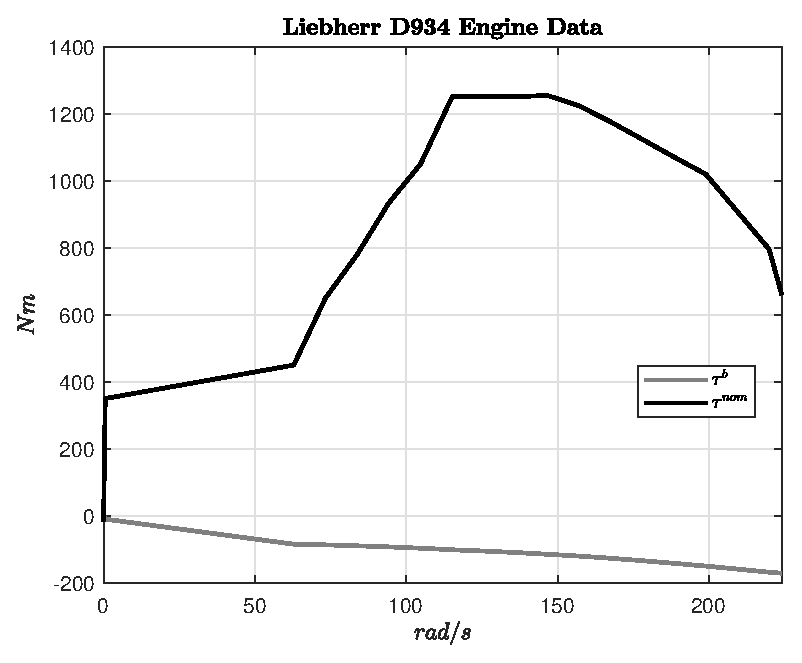
\includegraphics[width = 260pt, angle = 0, keepaspectratio]{figures/engine/engine_D934}
	\captionsetup{width=0.5\textwidth, font=small}		
	\caption{Engine model and control architecture.}
	\label{engine_curves}
\end{figure}
The control output $\theta$ is passed through a second order filter:
\begin{equation}
	\begin{aligned}
		\theta_f(s) = \frac{\omega_0^2}{s^2+2\zeta\omega_0s+\omega_0^2}\theta(s)
	\end{aligned}
\end{equation}
where $\zeta=1$ and $\omega_0=2\pi\SI{25}{\hertz}$.
\begin{figure}[H]
	\centering\includegraphics[width = 480pt, angle = 0, keepaspectratio]{figures/engine/diesel_engine_ctrl_2.eps}
	\captionsetup{width=0.5\textwidth, font=small}		
	\caption{Engine model and control architecture.}
	\label{engine_ctrl_1}
\end{figure}



\chapter{Vehicle Control architecture}
\section{Introduction}
The following document reports the description of some control systems used in the management of an heavy duty vehicle. The set of control systems specification can be summarized as follows
\begin{itemize} 
	\item Limit load control: the electronic control system regulates the engine speed and controls the driving speed depending on the required thrust force.
	\item Maximum speed limiter: controls the travel drive (speed) so that the set travel speed is not exceeded (e.g. downhill)
	\item Tracks synchronization control: adapts both sides of the tracks so that, for example, when driving straight ahead, the machine actually drives straight ahead.
	\item Pressure control: automatically reduces the pump adjustment when the high pressure limits are exceeded in order to prevent unnecessary energy loss via the pressure relief valves (e.g. in plowing operations).
\end{itemize} 

As first step a mathematical model of the hydrostatic power-train has been presented. The reason of the mathematical model has different scopes
\begin{itemize}
	\item find the fundamental motion equations of the system
	\item find the interconnection among the different dynamic equations
	\item find a possible model representation for model predictive control implementation
\end{itemize}   
%

\section{Nomenclature}
\begin{itemize}
	\item[--] $v_{track}^{R}$: speed of the right track in $\SI{}{\kilo\meter\per\hour}$.
	\item[--] $v_{track}^{L}$: speed of the right track in $\SI{}{\kilo\meter\per\hour}$.
	\item[--] $v_{track}^{sum}=v_{track}^{R}+v_{track}^{L}$: sum of the speed of the right and left track in $\SI{}{\kilo\meter\per\hour}$.
	\item[--] $v_{track}^{diff}=v_{track}^{R}-v_{track}^{L}$: sum of the difference between the right and left track $\SI{}{\kilo\meter\per\hour}$.
	\item[--] $v_{track}^{ref}\Big|_{R}$: speed set-point of the right track in $\SI{}{\kilo\meter\per\hour}$.
	\item[--] $v_{track}^{ref}\Big|_{L}$: speed set-point of the left track in $\SI{}{\kilo\meter\per\hour}$.
	\item[--] $v_{track}^{ref}\Big|_{R}^{max}$: maximum speed set-point of the right track in $\SI{}{\kilo\meter\per\hour}$.
	\item[--] $v_{track}^{ref}\Big|_{L}^{max}$: maximum speed set-point of the right track in $\SI{}{\kilo\meter\per\hour}$.
	\item[--] $\omega_l^R$: rotational speed of the follower (side which is connected to the track) of the right driver gear in $\SI{}{\radian\per\second}$.
	\item[--] $\omega_l^L$: rotational speed of the follower (side which is connected to the track) of the left driver gear in $\SI{}{\radian\per\second}$.
	\item[--] $\omega_m^R$: rotational speed of the driver (side which is connected to the hydraulic motor) of the right driver gear in $\SI{}{\radian\per\second}$.
	\item[--] $\omega_m^L$: rotational speed of the follower (side which is connected to the hydraulic motor) of the left driver gear in $\SI{}{\radian\per\second}$.
	\item[--] $\omega_m^{ref}$: hydraulic motor rotational speed set-point.
	\item[--] $n_{tg}$: drive gear ration.
	\item[--] $R_{tg}$: radius of the sprocket wheel connected to the track.
	\item[--] $V_m^{nom}$: nominal capacity of the hydraulic motor.
	\item[--] $V_p^{nom}$: nominal capacity of the hydraulic pump.
	\item[--] $\eta_m^{v}$: volumetric efficiency of the hydraulic motor.
	\item[--] $\eta_m^{m}$: mechanical efficiency of the hydraulic motor.
	\item[--] $\eta_p^{v}$: volumetric efficiency of the hydraulic pump.
	\item[--] $\eta_p^{m}$: mechanical efficiency of the hydraulic pump.
	
	\item[--] $d_p^R$: right drive-line,per unit pump volumetric displacement, where $d_p   \in [-d_p^\text{max},\ d_p^\text{max}]$, $d_p^\text{max}$ is in per unit.
	\item[--] $d_m^R$: right drive-line, per unit motor volumetric displacement, where $d_m\in [d_m^\text{min},\ d_m^\text{max}]$, $d_m^\text{max}$ and $d_m^\text{min}$ are in per unit.
	\item[--] $d_L$: left drive-line, per unit global volumetric displacement, where $d\in [-2d_p^\text{max}+d_m^\text{min},\ 2d_p^\text{max}-d_m^\text{min}]$, $d_p^\text{max}$ and $d_m^\text{min}$ are in per unit.
	\item[--] $d_p^L$: left drive-line, per unit pump volumetric displacement, where $d_p\in [-d_p^\text{max},\ d_p^\text{max}]$, $d_p^\text{max}$ is in per unit.
	\item[--] $d_m^L$: left drive-line, per unit motor volumetric displacement, where $d_m\in [d_m^\text{min},\ d_m^\text{max}]$, $d_m^\text{max}$ and $d_m^\text{min}$ are in per unit.
	\item[--] $\omega_e$: engine speed (also pump speed).
	\item[--] $\omega_e^{ref}$: engine rotational speed set-point.
	\item[--] $\tau_e$: engine torque in $\SI{}{\newton\meter}$.
	\item[--] $dir_R$: direction of the right track ($1$ or $-1$).
	\item[--] $dir_L$: direction of the left track ($1$ or $-1$).
	\item[--] $dir_S$: direction of the sum of the right and left track ($1$ or $-1$).
\end{itemize}

\section{Introduction}
In this document we propose a first draft of heavy duty vehicle control architecture based on independent feedback control loops which can be summarized as follows
\begin{itemize}
	\item A control loop which limits the maximum speed reached by the (\textit{sum}) sum of the tracks speed, where for \textit{sum} tracks speed it is intended $v_{track}^{sum} = v_{track}^{R} + v_{track}^{L}$. Supposing $v_{track}^{ref}\Big|_{sum}^{max} = v_{track}^{ref}\Big|_{R}^{max} + v_{track}^{ref}\Big|_{L}^{max}$ is the sum of the right and left maximum speed track reference (set-point). This control loop limits the maximum tracks  speed sum which e.g. we can assume the following value $v_{track}^{ref}\Big|_{sum}^{max} = \SI{11}{\kilo\meter\per\hour} + \SI{11}{\kilo\meter\per\hour} = \SI{22}{\kilo\meter\per\hour}$.
	\item A (\textit{diff}) difference tracks speed control or steering. Supposing $v_{track}^{ref}\Big|_{diff} = v_{track}^{ref}\Big|_{R} - v_{track}^{ref}\Big|_{L}$ the difference between the right and the left speed track reference (set-point) which results into a steering set-point. This control loop keeps the difference of the tracks speed to a given reference value and moreover saturates to a maximum value the steering speed.
	\item An \textit{engine anti-stall}. This control loop enables an automatic total volumetric displacement reduction in order to keep the engine at the given value of speed set-point. The effect of the anti-stall is to reduce both (for each side left and right) the current volumetric displacement according the maximum engine torque available at a given engine speed set-point. 
	\item Two \textit{pressure limitation} control loops. These two regulators automatically reduce the corresponding volumetric displacement in order to keep the relative driveline pressure below a given maximum value. E.g. we can assume a delta pressure limit value of $\Delta p^{lim}=\SI{420}{\bar}$.
\end{itemize}
\section{Control architecture}
\subsection{Introduction}
The power-train control which we are going to describe in next sections can be summarized as shown in Figure~\ref{control_overview}. Three groups of quantities can be distinguished 
\begin{itemize}
	\item[--] References
	\item[--] Measures
	\item[--] Control outputs
\end{itemize}  
\begin{figure}[H]
	\centering
	\includegraphics[width = 300pt, angle = 0, keepaspectratio]{figures/ctrl_architecture/powertrain_control_overview_1.eps}
	\captionsetup{width=0.5\textwidth, font=small}		
	\caption{Power-train control overview.}
	\label{control_overview}
\end{figure}

As \textit{References} are intended the right and left track speed targets, in $\Big[\SI{}{\kilo\meter\per\hour}\Big]$, and the engine rotational speed target, in $\Big[\SI{}{\per\minute}\Big]$.

As \textit{Measures} are intended the right and left track speeds, in $\Big[\SI{}{\kilo\meter\per\hour}\Big]$, the engine rotational speed, in $\Big[\SI{}{\per\minute}\Big]$, the right and left drive-line delta pressure, in $\Big[\SI{}{\bar}\Big]$, and the available engine torque, in $\Big[\SI{}{\newton\meter}\Big]$, derived from engine speed.

As \textit{Control outputs} are intended the volumetric displacements of the hydraulic pumps and hydraulic motors.

In order to simplify the control architecture the following mathematical objects are defined:
\begin{itemize}
	\item A \textbf{global} volumetric displacement (an object which include both motor and pump volumetric displacement) is created (see also Figure~\ref{total_volumetric_diplacementR} and Figure~\ref{total_volumetric_diplacementL}). Let $d$ be the \textbf{global} volumetric displacement, the terms $d_m$ and $d_p$ are derived as follows
	\begin{equation}
		\Biggl\{
		\begin{aligned}
			& d_m = d_m^{max} - \Big[\abs{d} - \abs{d_p}\Big] \quad \Rightarrow \quad d_m^{min}\le d_m \le d_m^{max} \\
			& d_p \quad \Rightarrow \quad -d_p^{max}\le d \le d_p^{max}
		\end{aligned}
	\end{equation}
	
	\begin{figure}[H]
		\centering
		\includegraphics[width = 350pt, angle = 0, keepaspectratio]{figures/ctrl_architecture/volumetric_displacement_construction_1a.eps}
		\captionsetup{width=0.5\textwidth, font=small}		
		\caption{Total volumetric displacement for the right drive-line.}
		\label{total_volumetric_diplacementR}
	\end{figure}
	
	\begin{figure}[H]
		\centering
		\includegraphics[width = 350pt, angle = 0, keepaspectratio]{figures/ctrl_architecture/volumetric_displacement_construction_1b.eps}
		\captionsetup{width=0.5\textwidth, font=small}		
		\caption{Total volumetric displacement for the left drive-line.}
		\label{total_volumetric_diplacementL}
	\end{figure}
	
	The construction of the \textbf{global} volumetric displacement is shown in Figure~\ref{global_ctrl1a} Figure~\ref{global_ctrl1b} and Figure~\ref{global_ctrl1c}.
	
	Let $d_R^{ctrl}$ and $d_L^{ctrl}$ be the volumetric displacements which are generated by the \textit{sum} and \textit{diff} tracks speed loops.
	
	Let $d_R^{ff}$ and $d_L^{ff}$ be the volumetric displacements which are generated as feed-forward from the tracks speed set-points as $v_{track}^{ref}\Big|_R$ and $v_{track}^{ref}\Big|_L$.
	
	The \textbf{global} volumetric displacements $d_R$ and $d_L$ are derived as follows
	\begin{equation}
		\Biggl\{
		\begin{aligned}
			& d_R = d_R^{ctrl} + d_R^{ff} \\
			& d_L = d_L^{ctrl} + d_L^{ff}
		\end{aligned}
	\end{equation}
	
	\item The \textbf{sum} and \textbf{diff} regulators are PI-based control loops, which require feedback defined as follows
	\begin{equation}
		% 	\begin{aligned}
			% 		& v_{track}^{ref}\Big|_{sum} = v_{track}^{ref}\Big|_{R} + v_{track}^{ref}\Big|_{L} \\[6pt]
			% 		& v_{track}^{ref}\Big|_{diff} = v_{track}^{ref}\Big|_{R} - v_{track}^{ref}\Big|_{L}
			% 	\end{aligned}
		\begin{aligned}
			& v_{track}^{sum} = v_{track}^{R} + v_{track}^{L} \\[6pt]
			& v_{track}^{diff} = v_{track}^{R} - v_{track}^{L}
		\end{aligned}
	\end{equation}
	where 
	\begin{equation}
		\begin{aligned}
			& v_{track}^{R} = \frac{1}{2}\Big[v_{track}^{sum} + v_{track}^{diff}\Big] \\[6pt]
			& v_{track}^{L} = \frac{1}{2}\Big[v_{track}^{sum} - v_{track}^{diff}\Big]
		\end{aligned}
	\end{equation}
	\item Two \textbf{global} volumetric displacement feed-forward as $d_R^{ff}$ and $d_L^{ff}$. The construction of the feed-forward terms are here reported. Let $v_{track}^{ref}$ be the speed track reference in $\SI{}{\meter\per\second}$ the equivalent hydraulic motor speed reference is given as follows
	\begin{equation}
		\omega_m^{ref} =\frac{v_{track}^{ref}}{R_{tg}}n_{tg}
	\end{equation}
	Let $\alpha_{ff}$ be the preliminary per unit volumetric displacement is given as follows
	\begin{equation}
		\alpha_{ff} =\frac{V_m^{nom}}{V_p^{nom}} \frac{1}{\eta_m^v\eta_p^v} \frac{\omega_m^{ref}}{\omega_e^{ref}}
	\end{equation}
	or also
	\begin{mybox}
		\begin{equation}
			\alpha_{ff} = \abs{\frac{1}{\eta_m^v\eta_p^v}\frac{1}{\omega_e^{ref}}\frac{V_m^{nom}}{V_p^{nom}} \frac{n_{tg}}{R_{tg}}v_{track}^{ref}}
		\end{equation}
	\end{mybox}
	the final formulation of the feed-forward $d^{ff}$ can be represented as follows
	\begin{equation}
		\boxed{d^{ff} = \left\lbrace \begin{aligned}
				& 2\,d_p^{max} - \frac{1}{\alpha_{ff}} \quad\text{if $\alpha_{ff} > d_p^{max}$} \\[6pt]
				& \alpha_{ff}  \quad\text{if $\alpha_{ff} \le d_p^{max}$}
			\end{aligned}\right. }
	\end{equation}
\end{itemize}

\subsection{Control layout}

In this section the global control layout is depicted. Some fundamental points are here reported.  

\begin{itemize}
	\item The main speed level is achieved by a feed-forward inputs $d_R^{ff}$ and $d_L^{ff}$, that means the main control is a open loop control. The external loops control just apply adjustment in order to avoid engine stall, over pressure and perform a synchronization among the two tracks. See Figure~\ref{global_ctrl1a}, Figure~\ref{global_ctrl1b} and Figure~\ref{global_ctrl1c}. 
	\item The speed track measure is not performed, but in its place, the driver gear (follower) rotational speeds $\omega_l^R$ and $\omega_l^L$ are measured. That means the overall quantities regarded $v_{track}$ will be converted (in algebraic way) into quantities of the form $\omega_l$, as follows
	\begin{itemize}
		\item The $\omega_l^{sum}=\omega_l^R+\omega_l^L$ control loop limits the maximum vehicle speed.
		\item The $\omega_l^{diff}=\omega_l^R-\omega_l^L$ control loop maintains both tracks speed at the same level when not steering is required, and adjust the $\omega_l^{diff}$ in case of steering demand.		
	\end{itemize}
	During straight driving the $\omega_l^{ref}\Big|_{diff}$ reference is set to zero.
	
	\item An engine anti-stall control loop is implemented, where the actual engine torque is compared with the torque limit curve $\tau_e(\omega_e)$ and the total volumetric displacement is properly compensated, see also Figure~\ref{global_ctrl1b}, Figure~\ref{global_ctrl1c} and Figure~\ref{engine_stall}. 
	\begin{figure}[H]
		\centering
		\includegraphics[width = 250pt, angle = 0, keepaspectratio]{figures/ctrl_architecture/engine_torque_compensation_2.eps}
		\captionsetup{width=0.5\textwidth, font=small}	e	
		\caption{Engine anti-stall implementation.}
		\label{engine_stall}
	\end{figure}
	\item The limit drive line delta pressure is also constrained by proper compensation of the total volumetric displacement, in order to limit its maximum value, when operative field condition permits it, see also Figure~\ref{global_ctrl1b}, Figure~\ref{global_ctrl1c} and Figure~\ref{pressure_limiter}. 
	\begin{figure}[H]
		\centering
		\includegraphics[width = 275pt, angle = 0, keepaspectratio]{figures/ctrl_architecture/delta_pressure_compensation_2.eps}
		\captionsetup{width=0.5\textwidth, font=small}		
		\caption{Drive line delta pressure limitation.}
		\label{pressure_limiter}
	\end{figure} 
\end{itemize}

\begin{figure}[H]
	\centering
	\includegraphics[width = 450pt, angle = 0, keepaspectratio]{figures/ctrl_architecture/global_control_1a.eps}
	\captionsetup{width=0.5\textwidth, font=small}	
	\caption{Steering and maximum speed limitation.}
	\label{global_ctrl1a}
\end{figure}
The global volumetric displacement is derived adding to the feed-forward and to the \textit{sum} and \textit{diff} control loops the \textit{field} compensations. For field here the engine anti-stall and over-pressure compensation is intended. Figure~\ref{compensation} shows the global volumetric displacement architecture comprehensive of the \textit{field} compensations.
\begin{figure}[H]
	\centering
	\includegraphics[width = 275pt, angle = 0, keepaspectratio]{figures/ctrl_architecture/compensation.eps}
	\captionsetup{width=0.5\textwidth, font=small}	
	\caption{Global volumetric displacement construction comprehensives of the compensations.}
	\label{compensation}
\end{figure}

\begin{figure}[H]
	\centering
	\includegraphics[width = 450pt, angle = 0, keepaspectratio]{figures/ctrl_architecture/global_control_1b.eps}
	\captionsetup{width=0.5\textwidth, font=small}	
	\caption{Architecture of the final volumetric displacement containing the engine stall and over-pressure compensation for right track.}
	\label{global_ctrl1b}
\end{figure}

\begin{figure}[H]
	\centering
	\includegraphics[width = 450pt, angle = 0, keepaspectratio]{figures/ctrl_architecture/global_control_1c.eps}
	\captionsetup{width=0.5\textwidth, font=small}	
	\caption{Architecture of the final volumetric displacement containing the engine stall and over-pressure compensation for left track.}
	\label{global_ctrl1c}
\end{figure}

\section{Case study}
The case study we are going to consider is a drive-train with the following data characteristics
\begin{itemize}
	\item $V_m^{nom} = \SI{252.8}{\cubic\centi\meter}$
	\item $V_p^{nom} = \SI{147.2}{\cubic\centi\meter}$
	\item $R = \SI{0.44056}{\meter}$
	\item $n_{tg} = n_1/n_2 = \SI{41.4}{}$
	\item $v_{tr}^{max} = \SI{11.0}{\kilo\meter\per\hour}$
	\item $\eta_p^m=\SI{0.909}{}$
	\item $\eta_p^v=\SI{0.959}{}$
	\item $\eta_m^m=\SI{0.939}{}$
	\item $\eta_m^v=\SI{0.943}{}$
\end{itemize}


\subsection{Simulation results}

\subsubsection{Scenario 1}
In this scenario we are considering the following case
\begin{itemize}
	\item Straight driving.
	\item Not homogeneous viscosity load on tracks. 
	\item The total amount of load is enough to stall the engine.
	\item The maximum per drive-line load doesn't exceed the maximum admissible delta pressure.
\end{itemize} 
\begin{figure}[H]
	\centering
	\includegraphics[width = 450pt, angle = 0, keepaspectratio]{figures/ctrl_architecture/test_scenario_1.eps}
	\captionsetup{width=0.5\textwidth, font=small}	
	\caption{Description of the test scenario 1.}
	\label{test_scenario_1}
\end{figure}

\begin{figure}[H]
	\centering
	\begin{subfigure}{.5\textwidth}
		\centering
		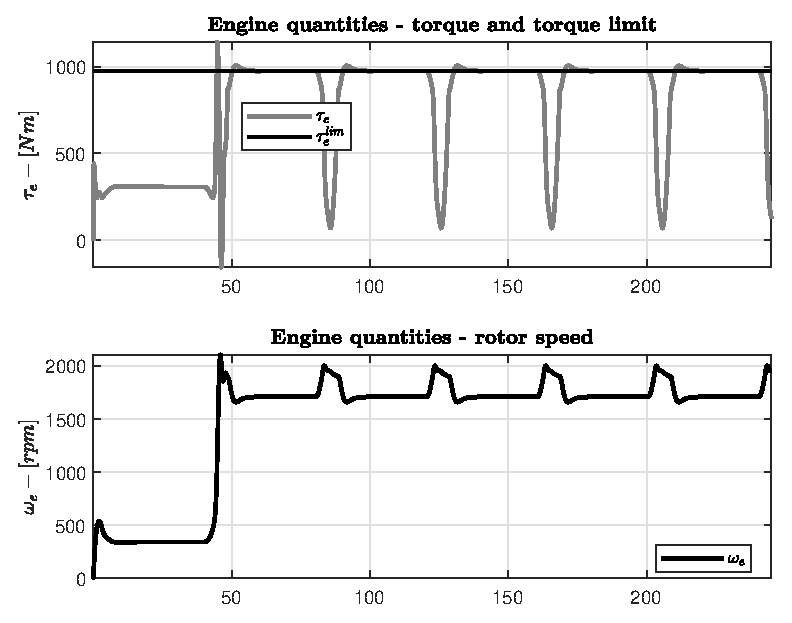
\includegraphics[width = 200pt, angle=0, keepaspectratio]{figures/ctrl_architecture/load_case_1/engine_data_1.eps}
		\captionsetup{width=.75\textwidth}
		\caption{Engine data.}
		\label{}
	\end{subfigure}%
	\begin{subfigure}{.5\textwidth}
		\centering
		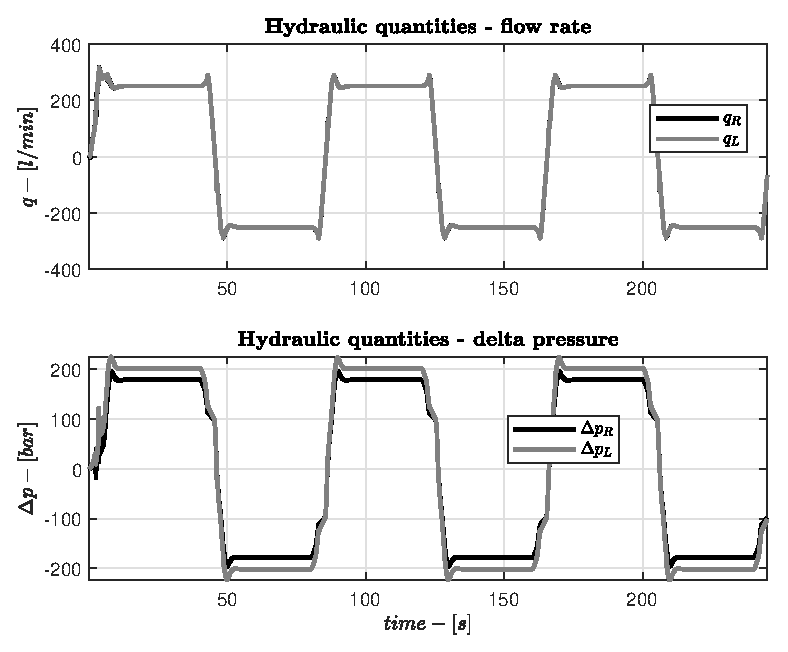
\includegraphics[width = 200pt, angle=0, keepaspectratio]{figures/ctrl_architecture/load_case_1/hydro_data_1.eps}
		\captionsetup{width=.75\textwidth}
		\caption{Hydrostatic drive-line data.}
		\label{}
	\end{subfigure}
	\caption{Simulation results scenario 1.}
	\label{}
\end{figure}
\begin{figure}[H]
	\centering
	\begin{subfigure}{.5\textwidth}
		\centering
		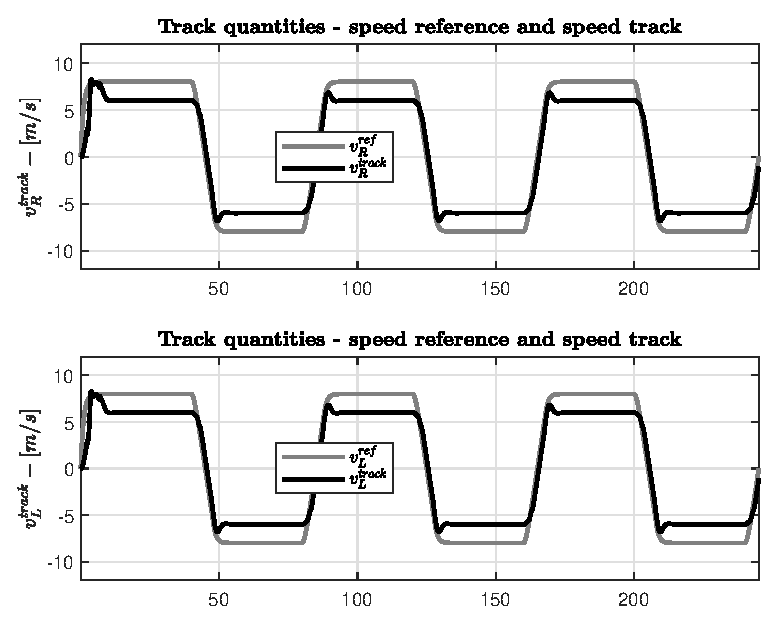
\includegraphics[width = 200pt, angle=0, keepaspectratio]{figures/ctrl_architecture/load_case_1/track_data_1.eps}
		\captionsetup{width=.75\textwidth}
		\caption{Speed tracks tracking performance.}
		\label{}
	\end{subfigure}%
	\begin{subfigure}{.5\textwidth}
		\centering
		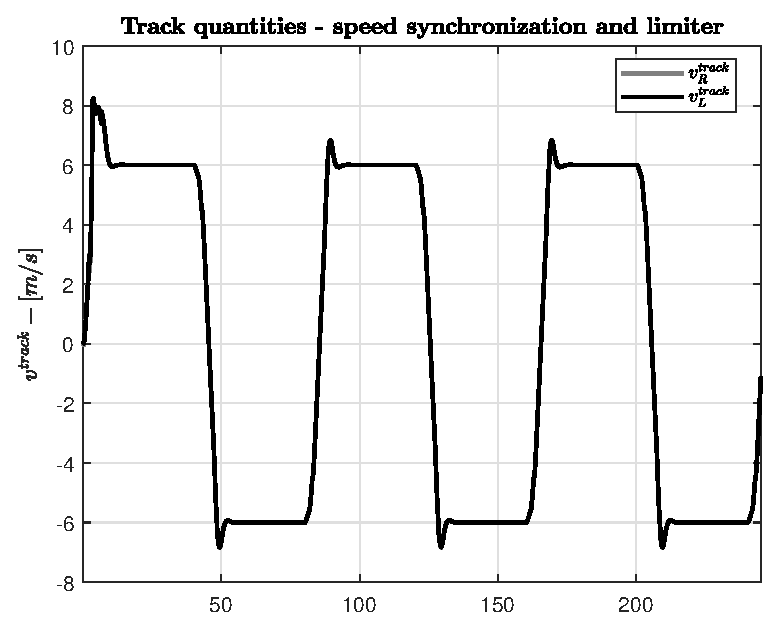
\includegraphics[width = 200pt, angle=0, keepaspectratio]{figures/ctrl_architecture/load_case_1/track_data_2.eps}
		\captionsetup{width=.75\textwidth}
		\caption{Speed tracks synchronization and maximum speed limiter.}
		\label{}
	\end{subfigure}
	\caption{Simulation results scenario 1.}
	\label{}
\end{figure}
\begin{figure}[H]
	\centering
	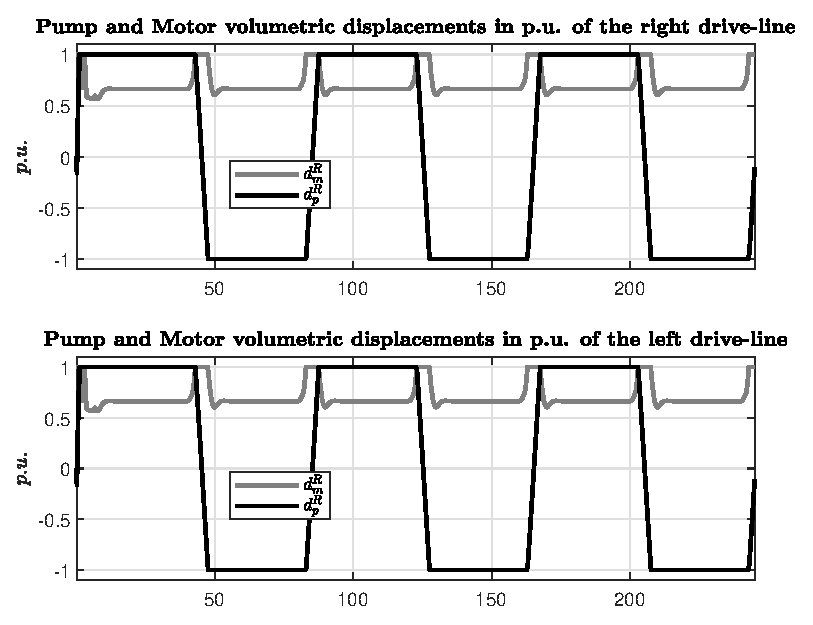
\includegraphics[width = 300pt, angle=0, keepaspectratio]{figures/ctrl_architecture/load_case_1/volumetric_displacements.eps}
	\captionsetup{width=.75\textwidth}
	\caption{Volumetric displacements.}
	\label{}
\end{figure}

\subsubsection{Scenario 2}
In this scenario we are considering the following case
\begin{itemize}
	\item Straight driving.
	\item Not homogeneous viscosity load on tracks. 
	\item The total amount of load is enough to stall the engine.
	\item The maximum load on drive-line one (Right) exceed the maximum admissible delta pressure.
\end{itemize} 
\begin{figure}[H]
	\centering
	\includegraphics[width = 450pt, angle = 0, keepaspectratio]{figures/ctrl_architecture/test_scenario_2.eps}
	\captionsetup{width=0.5\textwidth, font=small}	
	\caption{Description of the test scenario 2.}
	\label{test_scenario_2}
\end{figure}
\begin{figure}[H]
	\centering
	\begin{subfigure}{.5\textwidth}
		\centering
		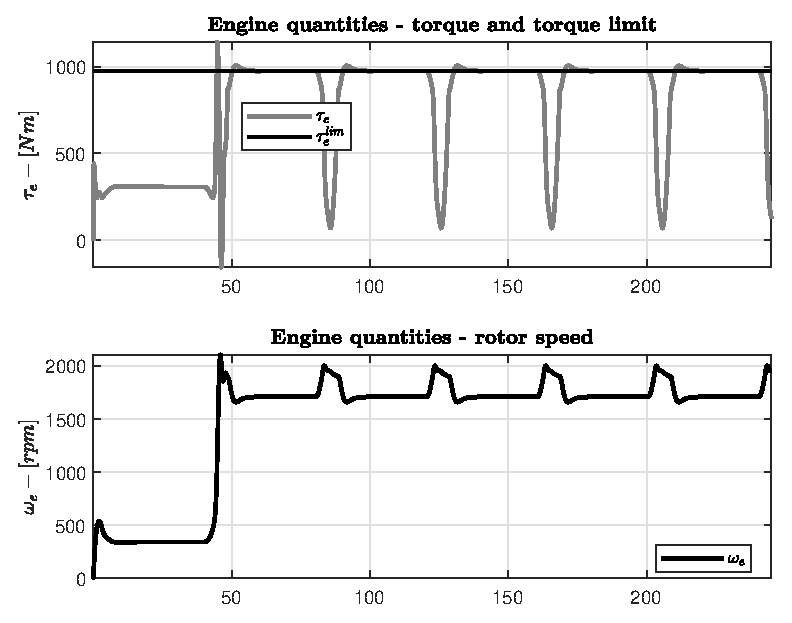
\includegraphics[width = 200pt, angle=0, keepaspectratio]{figures/ctrl_architecture/load_case_1/engine_data_1.eps}
		\captionsetup{width=.75\textwidth}
		\caption{Engine data.}
		\label{}
	\end{subfigure}%
	\begin{subfigure}{.5\textwidth}
		\centering
		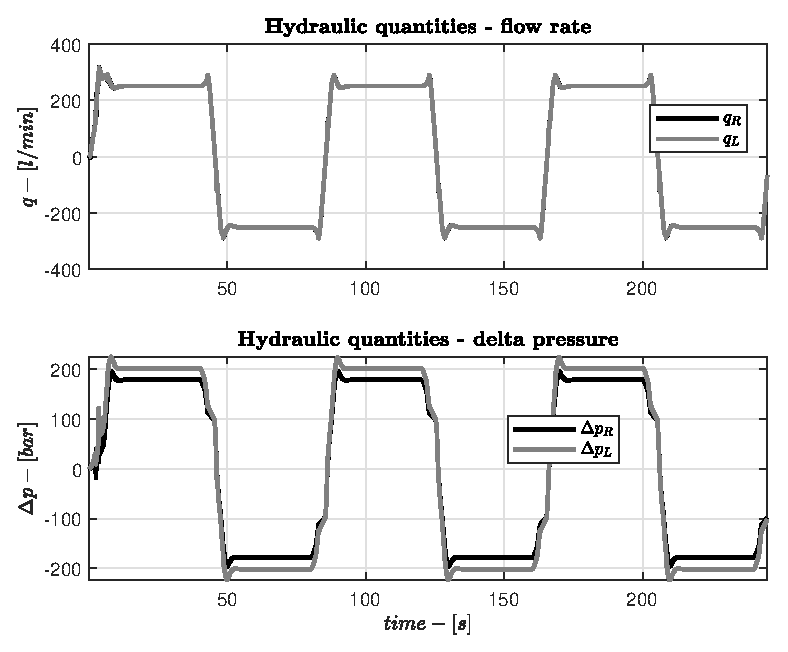
\includegraphics[width = 200pt, angle=0, keepaspectratio]{figures/ctrl_architecture/load_case_1/hydro_data_1.eps}
		\captionsetup{width=.75\textwidth}
		\caption{Hydrostatic drive-line data.}
		\label{}
	\end{subfigure}
	\caption{Simulation results scenario 2.}
	\label{}
\end{figure}
\begin{figure}[H]
	\centering
	\begin{subfigure}{.5\textwidth}
		\centering
		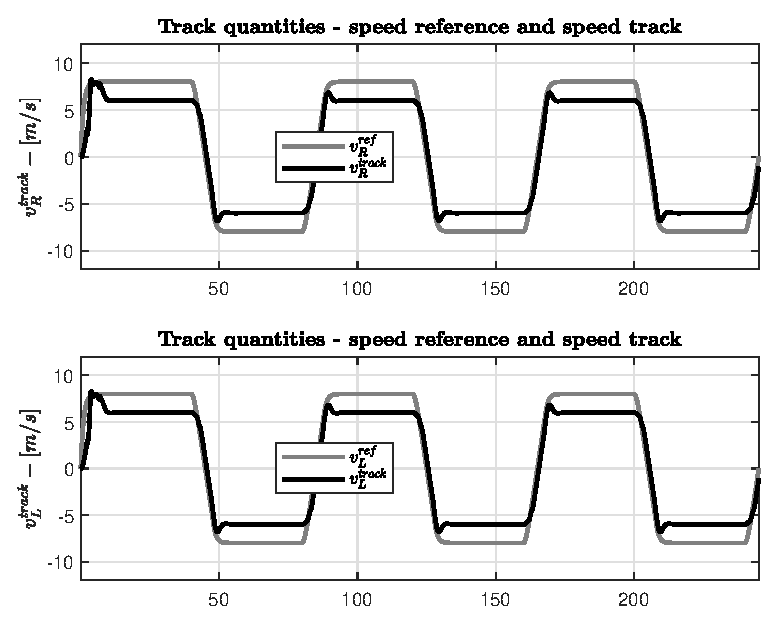
\includegraphics[width = 200pt, angle=0, keepaspectratio]{figures/ctrl_architecture/load_case_1/track_data_1.eps}
		\captionsetup{width=.75\textwidth}
		\caption{Speed tracks tracking performance.}
		\label{}
	\end{subfigure}%
	\begin{subfigure}{.5\textwidth}
		\centering
		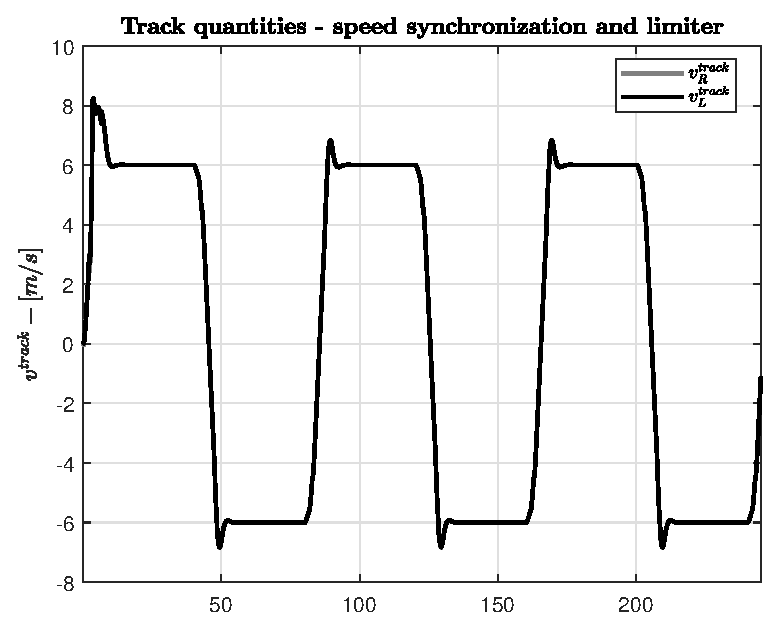
\includegraphics[width = 200pt, angle=0, keepaspectratio]{figures/ctrl_architecture/load_case_1/track_data_2.eps}
		\captionsetup{width=.75\textwidth}
		\caption{Speed tracks synchronization and maximum speed limiter.}
		\label{}
	\end{subfigure}
	\caption{Simulation results scenario 2.}
	\label{}
\end{figure}
\begin{figure}[H]
	\centering
	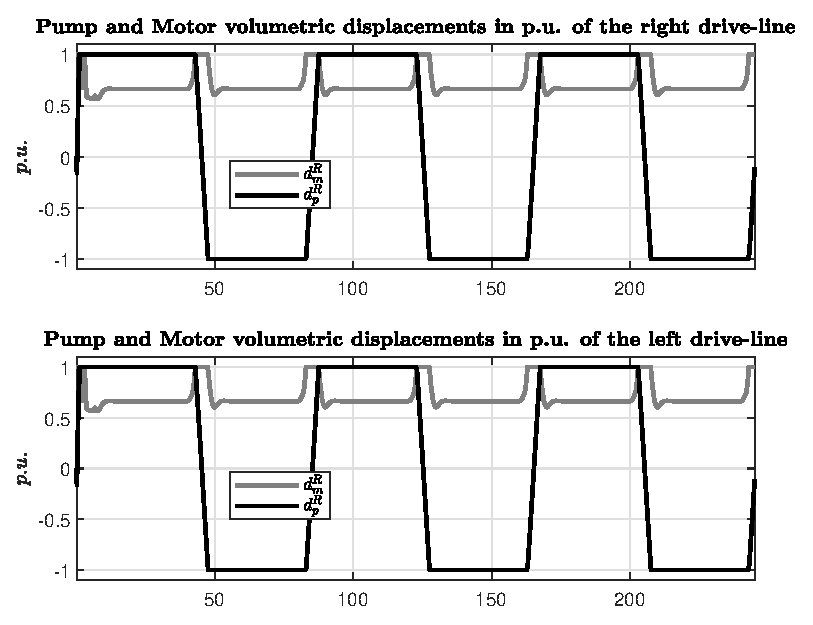
\includegraphics[width = 300pt, angle=0, keepaspectratio]{figures/ctrl_architecture/load_case_1/volumetric_displacements.eps}
	\captionsetup{width=.75\textwidth}
	\caption{Volumetric displacements.}
	\label{}
\end{figure}

\subsubsection{Scenario 3}
In this scenario we are considering the following case
\begin{itemize}
	\item Straight driving.
	\item Homogeneous negative load on both track (downhill scenario). 
	\item The maximum negative load brings the vehicle in over-speed condition (over-speed management).
\end{itemize} 
\begin{figure}[H]
	\centering
	\includegraphics[width = 450pt, angle = 0, keepaspectratio]{figures/ctrl_architecture/test_scenario_3.eps}
	\captionsetup{width=0.5\textwidth, font=small}	
	\caption{Description of the test scenario 3.}
	\label{test_scenario_3}
\end{figure}
\begin{figure}[H]
	\centering
	\begin{subfigure}{.5\textwidth}
		\centering
		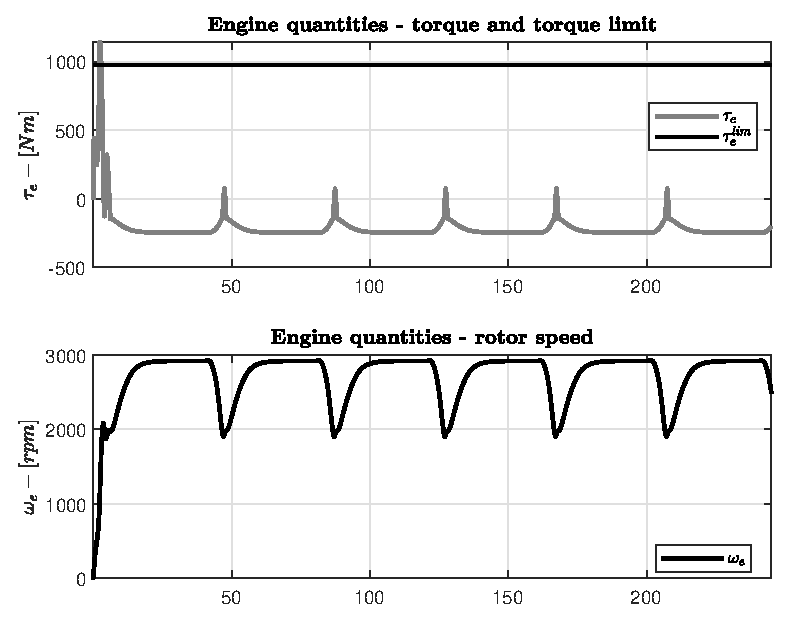
\includegraphics[width = 200pt, angle=0, keepaspectratio]{figures/ctrl_architecture/load_case_3/engine_data_1.eps}
		\captionsetup{width=.75\textwidth}
		\caption{Engine data.}
		\label{}
	\end{subfigure}%
	\begin{subfigure}{.5\textwidth}
		\centering
		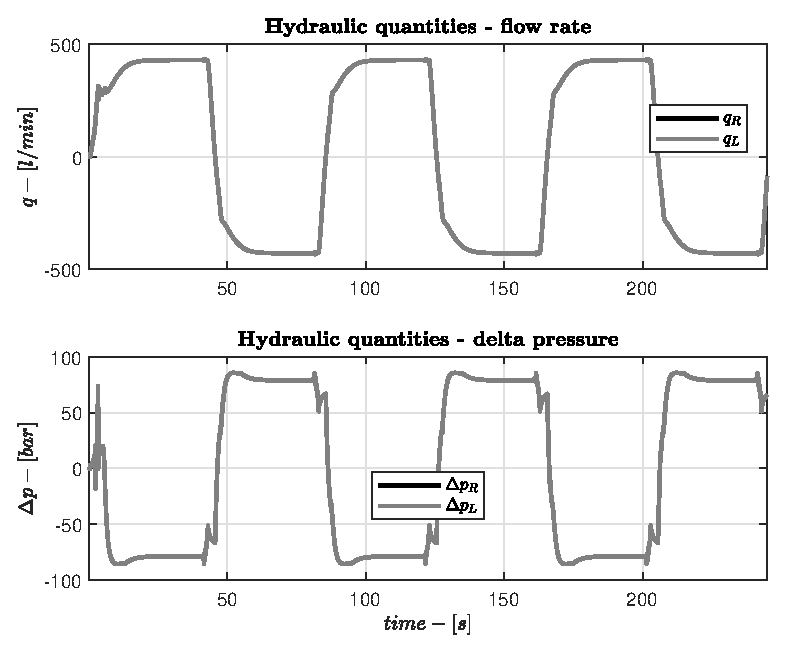
\includegraphics[width = 200pt, angle=0, keepaspectratio]{figures/ctrl_architecture/load_case_3/hydro_data_1.eps}
		\captionsetup{width=.75\textwidth}
		\caption{Hydrostatic drive-line data.}
		\label{}
	\end{subfigure}
	\caption{Simulation results scenario 3.}
	\label{}
\end{figure}
\begin{figure}[H]
	\centering
	\begin{subfigure}{.5\textwidth}
		\centering
		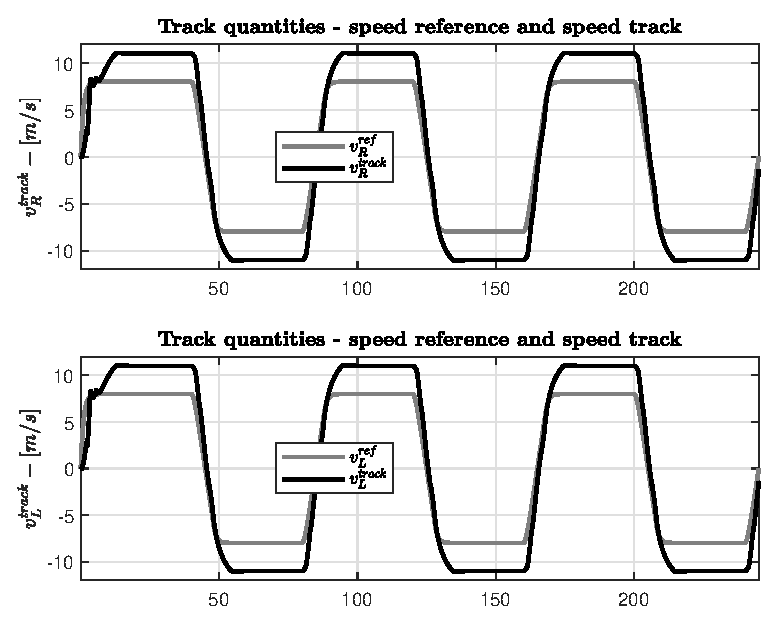
\includegraphics[width = 200pt, angle=0, keepaspectratio]{figures/ctrl_architecture/load_case_3/track_data_1.eps}
		\captionsetup{width=.75\textwidth}
		\caption{Speed tracks tracking performance.}
		\label{}
	\end{subfigure}%
	\begin{subfigure}{.5\textwidth}
		\centering
		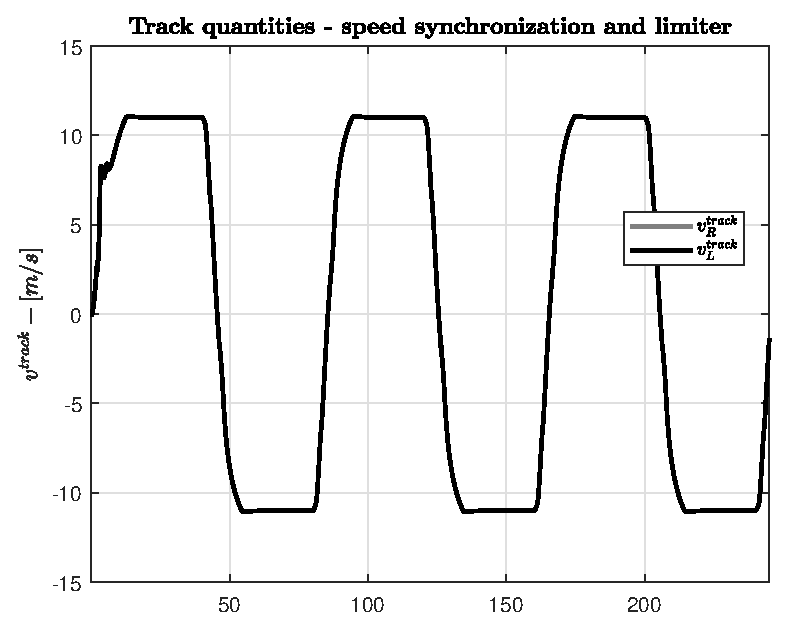
\includegraphics[width = 200pt, angle=0, keepaspectratio]{figures/ctrl_architecture/load_case_3/track_data_2.eps}
		\captionsetup{width=.75\textwidth}
		\caption{Speed tracks synchronization and maximum speed limiter.}
		\label{}
	\end{subfigure}
	\caption{Simulation results scenario 3.}
	\label{}
\end{figure}
\begin{figure}[H]
	\centering
	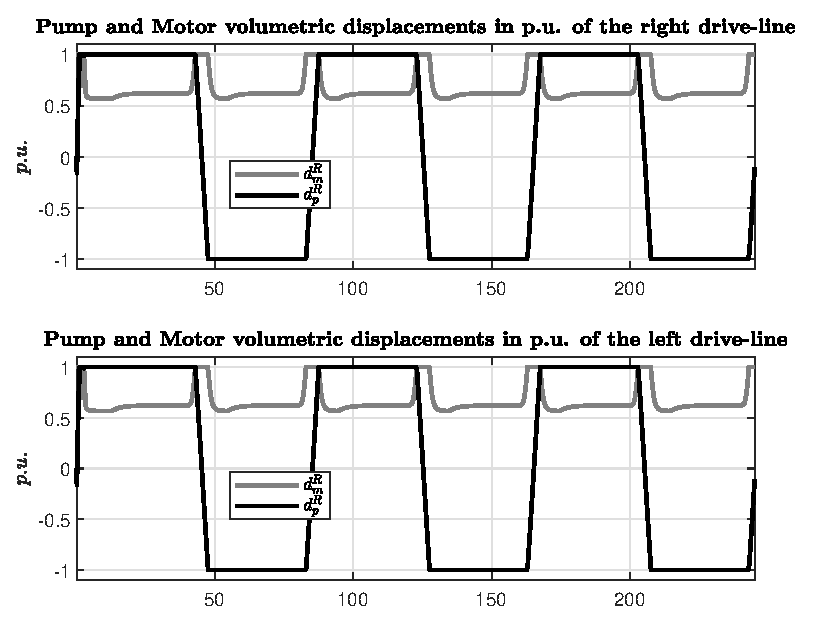
\includegraphics[width = 300pt, angle=0, keepaspectratio]{figures/ctrl_architecture/load_case_3/volumetric_displacements.eps}
	\captionsetup{width=.75\textwidth}
	\caption{Volumetric displacements.}
	\label{}
\end{figure}

\subsubsection{Scenario 4}
In this scenario we are considering the following case
\begin{itemize}
	\item Steering driving.
	\item Not homogeneous viscosity load on tracks. 
	\item The total amount of load is enough to stall the engine.
	\item The maximum load on drive-line one (Right) exceed the maximum admissible delta pressure.
\end{itemize} 
\begin{figure}[H]
	\centering
	\includegraphics[width = 450pt, angle = 0, keepaspectratio]{figures/ctrl_architecture/test_scenario_4.eps}
	\captionsetup{width=0.5\textwidth, font=small}	
	\caption{Description of the test scenario 4.}
	\label{test_scenario_4}
\end{figure}
\begin{figure}[H]
	\centering
	\begin{subfigure}{.5\textwidth}
		\centering
		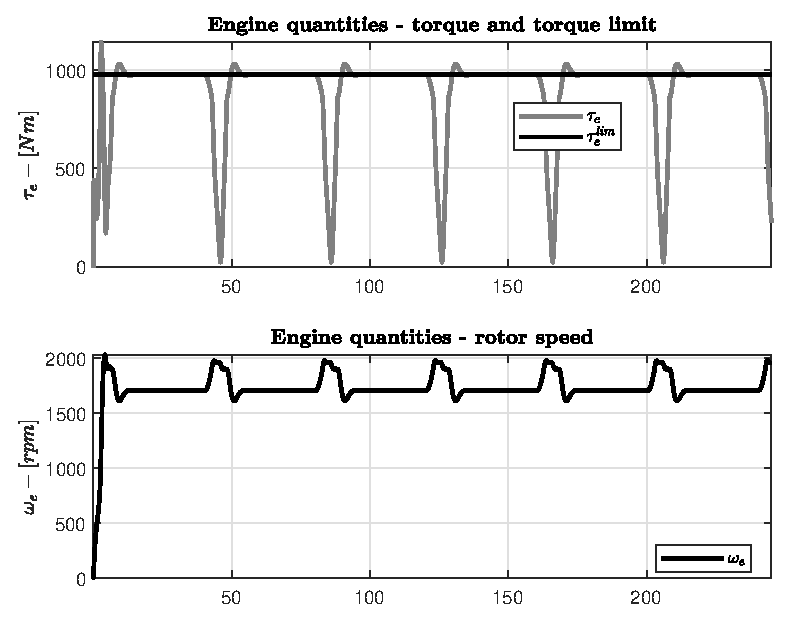
\includegraphics[width = 200pt, angle=0, keepaspectratio]{figures/ctrl_architecture/load_case_4/engine_data_1.eps}
		\captionsetup{width=.75\textwidth}
		\caption{Engine data.}
		\label{}
	\end{subfigure}%
	\begin{subfigure}{.5\textwidth}
		\centering
		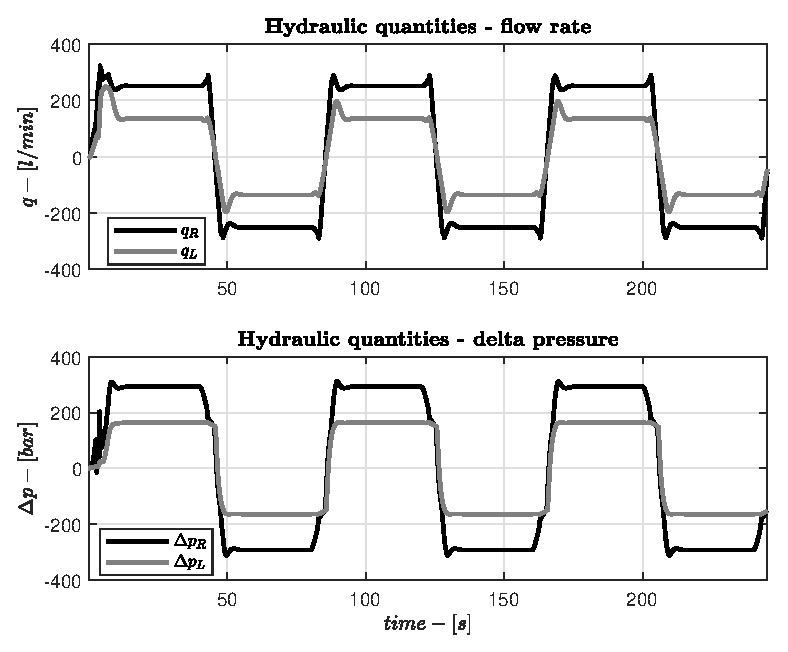
\includegraphics[width = 200pt, angle=0, keepaspectratio]{figures/ctrl_architecture/load_case_4/hydro_data_1.eps}
		\captionsetup{width=.75\textwidth}
		\caption{Hydrostatic drive-line data.}
		\label{}
	\end{subfigure}
	\caption{Simulation results scenario 3.}
	\label{}
\end{figure}
\begin{figure}[H]
	\centering
	\begin{subfigure}{.5\textwidth}
		\centering
		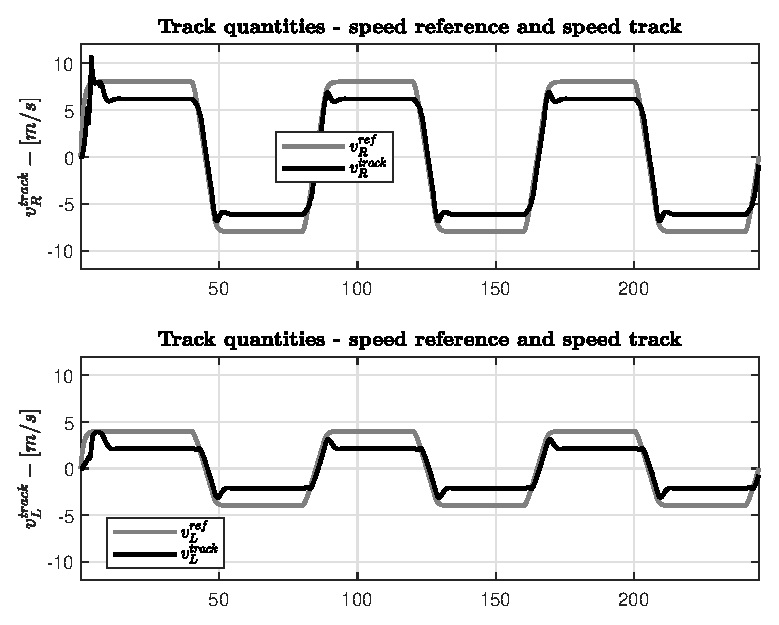
\includegraphics[width = 200pt, angle=0, keepaspectratio]{figures/ctrl_architecture/load_case_4/track_data_1.eps}
		\captionsetup{width=.75\textwidth}
		\caption{Speed tracks tracking performance.}
		\label{}
	\end{subfigure}%
	\begin{subfigure}{.5\textwidth}
		\centering
		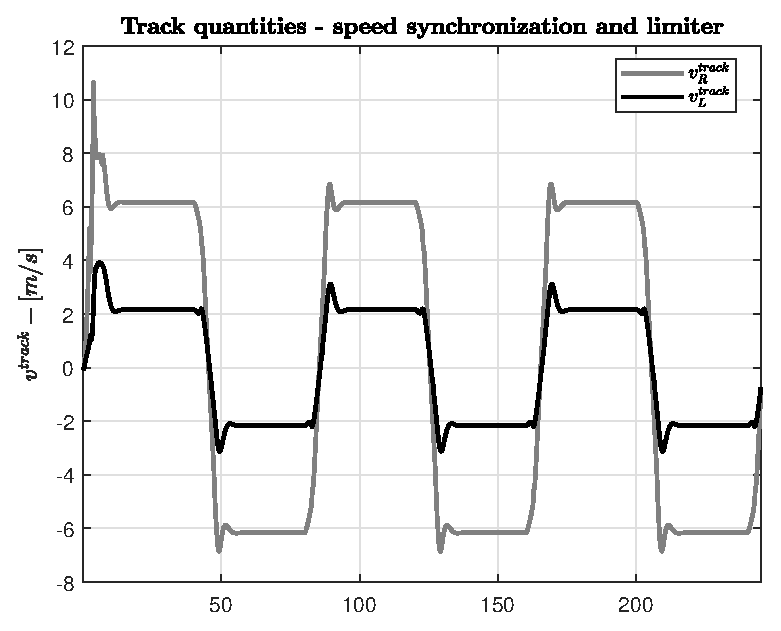
\includegraphics[width = 200pt, angle=0, keepaspectratio]{figures/ctrl_architecture/load_case_4/track_data_2.eps}
		\captionsetup{width=.75\textwidth}
		\caption{Speed tracks synchronization and maximum speed limiter.}
		\label{}
	\end{subfigure}
	\caption{Simulation results scenario 3.}
	\label{}
\end{figure}
\begin{figure}[H]
	\centering
	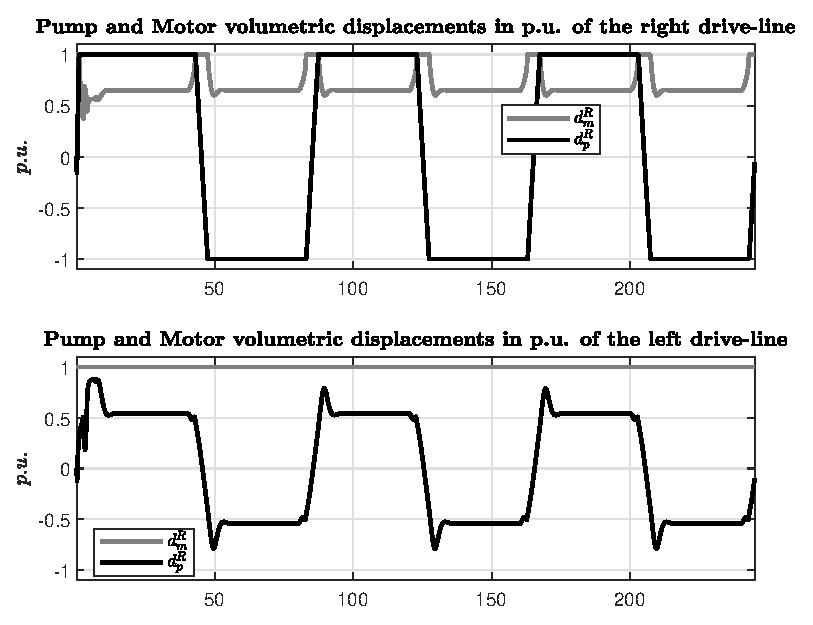
\includegraphics[width = 300pt, angle=0, keepaspectratio]{figures/ctrl_architecture/load_case_4/volumetric_displacements.eps}
	\captionsetup{width=.75\textwidth}
	\caption{Volumetric displacements.}
	\label{}
\end{figure}




\part{Electrification of an Hydrostatic Power-train}
\chapter{Introduction}
The electrification of the power-train consists in the replacement of the diesel engine and of the hydrostatic transmissions by a set of electrical equipment, consisting on:
\begin{itemize}
	\item A fuel cell and its control system.
	\item A dc/dc converter and its control system.
	\item A battery and its battery management system.
	\item A braking unit and its control system.
	\item An inverter unit and its control system. 
	\item A permanent magnet synchronous motor (PMSM). 
\end{itemize} 
Figure~\ref{electrical_pt_1} shows the whole layout.
\begin{figure}[H]
	\centering
	\includegraphics[width = 450pt, angle = 0, keepaspectratio]{figures/electrical_pt_1.eps}
	\captionsetup{width=0.5\textwidth, font=small}		
	\caption{Electrical layout overview.}
	\label{electrical_pt_1}
\end{figure}
The dimensioning of the electrical equipment shall start from the torque-speed limit curve shown in Figure~\ref{limit_curves1}, where the sizing of the PMSM is directly affected. In additional, the motor control strategy (inverter control) which has been accounted will affect also the dimensioning of the PMSM. The whole design is also strongly bounded by the constraints given by the semiconductor components which must be selected around a given set of industrial products. 

In the following we will describe the physical model around each component, which the power-train consist of. We will start from the power source, which means the PEM fuel-cell, to arrive to the Lithium-ion battery and its DC/DC power supply equipment. 

The last component is the \textbf{driver} unit which consists of an inverter, a PMSM and the motor control unit which plays a fundamental role in the whole design.

\chapter{Internal design of a permanent magnet synchronous machine (PMSM)}

\section{Preliminary dimensioning}

According to the hydrostatic performance results, shown in Figure~\ref{limit_curves1}, the design of the PMSM, one for each drive line, shall be sized according the following constraints:\\
\begin{itemize}
	\item $\hat{v}_{dc}=\hat{E}_{ph}\sqrt{3}=\SI{800}{\volt}$   
	\item $\hat{\omega}_{m}=\SI{3100}{\per\minute}$
	\item $\hat{\tau}_{m}=\SI{1600}{\newton\meter}$\\
\end{itemize}
where $\hat{E}_{ph}$ is the maximum phase peak voltage at no-load (no-current).
The constraint $\hat{E}_{ph}$ is the maximum phase peak voltage occurs at maximum rotor speed in the case of no-load (or in general the inverter is not in the operative mode). The voltage limit $\hat{E}_{ph}$ is correlated to the maximum DClink voltage permitted (with proper margin of safety) and the maximum phase peak voltage $\hat{E}_{ph}$ is directly correlated to the maximum rotor speed as follows
\begin{equation}
	\begin{aligned}
		\hat{E}_{ph} = p\hat{\omega}_m\hat{\psi}^M
	\end{aligned}
\end{equation}
where $p$ is the number of pole pairs and $\hat{\psi}^M$ is the rotor permanent magnet flux linked to the stator winding along the $\tau/2$ region as shown in Figure~\ref{pmsm_drawing_2}.
The equation of the torque as function of the phase current $\hat{i}_{q}$ (here we suppose that $\hat{i}_{ph}=\hat{i}_{q}$) is given as follows
\begin{equation}
	\begin{aligned}
		\hat{\tau}_{m} = \frac{3}{2}p\hat{i}_q\hat{\psi}^M
	\end{aligned}
\end{equation}
Considering the following constraints
\begin{itemize}
	\item $\hat{v}_{dc}=\hat{E}_{ph}\sqrt{3}=\SI{800}{\volt}$
	\item $\hat{\omega}_{m}=\SI{3100}{\per\minute}$
	\item $\hat{\tau}_{m}=\SI{1600}{\newton\meter}$
	\item $D_{tg} = \SI{41.4}{}$
\end{itemize}
we obtain
\begin{equation}
	\hat{\psi}^{M}=\frac{\hat{v}_{dc}}{\sqrt{3} p \hat{\omega}_{m}}=\SI{0.356}{\weber}
\end{equation}
\begin{equation}
		\hat{i}_{q}=\frac{2}{3}\frac{\hat{\tau}_m}{p \hat{\psi}^{M}}=\frac{2}{\sqrt{3}}\frac{\hat{\tau}_m\hat{\omega}_m}{\hat{v}_{dc}}=\SI{750}{\ampere} \quad\text{for $\hat{v}_{dc}=\SI{800}{\volt}$}
\end{equation} 
the maximum permissible dc voltage will affect the sizing of the pmsm.
\begin{equation}
	\begin{aligned}
&\hat{i}_{q}=\frac{2}{\sqrt{3}}\frac{\hat{\tau}_m\hat{\omega}_m}{\hat{v}_{dc}}=\SI{750}{\ampere} \quad\text{for $\hat{v}_{dc}=\SI{800}{\volt}$} \\[6pt]
&\hat{i}_{q}=\frac{2}{\sqrt{3}}\frac{\hat{\tau}_m\hat{\omega}_m}{\hat{v}_{dc}}=\SI{480}{\ampere} \quad\text{for $\hat{v}_{dc}=\SI{1250}{\volt}$}
	\end{aligned}
\end{equation} 
all quantities here are in peak values (not-rms).
At this stage the two fundamental quantities have been sized: a nominal current of the inverter and pmsm ($\hat{i}_{q}$) and the nominal magnetic flux linked to the winding ($\hat{\psi}^{M}$) which will affect the geometric sizing of the motor.
\begin{figure}[H]
	\centering
	\includegraphics[width = 400pt, keepaspectratio]{figures/driver_1_fault.eps}
	\caption{Inverter fault representation.}
	\label{driver_1_fault}
\end{figure}
The two preliminaries design quantities have been calculated supposing a maximum motor terminal voltage of $\SI{566}{\volt}$ (line-rms). The designed current of $\SI{750}{\ampere}$ is a value which will affect the thermal behaviour of the motor and it seems not to be of practical use. Hence the design of the PMSM will be carried out imposing an higher maximum terminal voltage  

\section{Basic of interior machine design}

%\subsection{Magnetic design}
%
%\subsection{Electrical design  }


Before to start with the geometric sizing of the motor we want to select the material we intend to use.
\begin{itemize}
	\item The stator and rotor are made by a pack of laminated crystal-oriented electrical steel: \textbf{Isovac 400 65A}.
	\item The rotor magnets are made by a NdFeB (\textbf{NdFe35}) considering a remain magnetic induction of  $B_r=\SI{1.35}{\weber\per\square\meter}$ at the temperature of $T=\SI{20}{\celsius}$
	%	\item The stator wingdings are made by \textbf{aluminum} wire insulated by \textbf{mica}. Where $\rho_{Al}=\SI{0.0286}{\ohm\square\milli\meter\per\meter}$.
	\item The stator windings are made by \textbf{aluminium} wire insulated by \textbf{mica}. Where $\rho_{Cu}=\SI{0.0275}{\ohm\square\milli\meter\per\meter}$ at $T=\SI{20}{\celsius}$.
\end{itemize}
To size the pmsm we started from a “done” geometry (in term of rotor and stator diameters) e we scale the length of the motor according to the value of permanent magnet flux linked to the stator winding.
\begin{figure}[H]
	\centering
	\includegraphics[width = 300pt, keepaspectratio]{figures/magnet_load.eps}
	\caption{Permanent magnet operating point.}
	\label{magnet_load}
\end{figure}
%\begin{figure}[H]
%	\centering
%	\includegraphics[width = 350pt, keepaspectratio]{figures/coil_magnet_circuit_1.eps}
%	\caption{Simplified representation of the PMSM along a pole.}
%	\label{pmsm_design_1}
%\end{figure}
%\begin{figure}[H]
%	\centering
%	\includegraphics[width = 175pt, keepaspectratio]{figures/pmsm_drawing_6.eps}
%	\caption{Integration path of the Ampere's law used to estimated the air-gap magnetic field density.}
%	\label{pmsm_drawing_4}
%\end{figure}
The rotor magnetic flux circuit can be approximated as reported in Figure~\ref{pmsm_design_1} and Figure~\ref{magnet_load} by a simple magnetic circuit by the assumption of infinity permeability of the rotor and stator core. Applying Ampere's and Gauss's laws, to the case of no-current at the stator winding, we obtain the following constitutive equations\footnote{$B_{m}h_m L_\text{stack} = B_g\frac{\pi D_r}{4p}L_\text{stack} \Rightarrow B_{m}h_m = B_g\frac{\pi D_r}{4p}$}
%\begin{equation}\label{magnetic_circuit_1}
%	\begin{aligned}
	%		&B_{m}h_m = B_g\frac{\pi D_r}{4p} \\[6pt]
	%		&2H_mt_m+2H_gg=0
	%	\end{aligned}
%\end{equation}
\begin{align}\label{magnetic_circuit_1}
	&2 B_{m}h_m = B_g\frac{\pi D_r}{2p} \\[6pt]
	&2H_mt_m+2H_gg=0
\end{align}
from Figure~\ref{magnet_load} we can derive that 
\begin{equation}
	\begin{aligned}
		&B_m = B_r + H_m\mu_r^m\mu_0 \Rightarrow H_m = \frac{B_m-B_r}{\mu_r^m\mu_0}
	\end{aligned}
\end{equation}
hence Eq.~\eqref{magnetic_circuit_1} can be written as follows
\begin{equation}
	\begin{aligned}
		&\frac{B_{m}-B_r}{\mu_r^m\mu_0}t_m + \frac{B_g}{\mu_0}g=0 \quad\Rightarrow\quad B_g=B_r \Big/ \Big(\frac{\pi D_r}{4p\,h_m}+\frac{g}{t_m}\mu_r^m\Big)
	\end{aligned}
\end{equation}
where the permanent magnet flow linked to the stator winding is given as follows
\begin{equation}
	\begin{aligned}
		\psi^M=B_g\frac{D_r\pi}{4p}L_{stack}N
	\end{aligned}
\end{equation}
From the the air-gap magnetic field density $B_g$ is also possible to evaluate the magnetic field density in the stator tooth and in the stator yoke applying Gauss's law.
Figure~\ref{pmsm_drawing_3} shows the behaviour of the $\psi^M$ flow-stream along the magnetic circuit. 
%\begin{figure}[H]
%	\centering
%	\includegraphics[width = 260pt, keepaspectratio]{figures/pmsm/pm_flows.eps}
%	\captionsetup{width=0.5\textwidth, font=small}
%	\caption{PMSM - description of the streamline flow of the magnetic flow $\psi^M$}
%	\label{pmsm_drawing_3}
%\end{figure}
\begin{figure}[H]
	\centering
	\begin{subfigure}{.5\textwidth}
		\centering
		\includegraphics[width = 200pt, keepaspectratio]{figures/coil_magnet_circuit_1.eps}
		\captionsetup{width=0.5\textwidth, font=small}		
		\caption{Simplified representation of the PMSM along a pole.}
		\label{pmsm_drawing_3}
	\end{subfigure}%
	\begin{subfigure}{.5\textwidth}
		\centering
		\includegraphics[width = 200pt, keepaspectratio]{figures/pmsm/ampere_law2.eps}
		\captionsetup{width=0.5\textwidth, font=small}		
		\caption{Integration path of the Ampere's law used to estimated the air-gap magnetic field density.}
		\label{}
	\end{subfigure}
	\caption{Magnetic circuit representation}
	\label{pmsm_design_1}
\end{figure}

The whole PMSM is depicted in Figure~\ref{pmsm_drawing_1} which correspond to an eight poles forty eight slots.
Following the drawing reported in Figure~\ref{pmsm_drawing_2} we make a list of geometric parameters as follows


\section{16 poles 12 slots solution}
Figure~\ref{pmsm_drawing_2} and Figure~\ref{pmsm_drawing_1} show the whole geometric parameters which are involved in the design of the PMSM. The fixed geometric parameter as well as material properties are here summarized
\begin{itemize}
	\item Number of slots $N_{sl}=12$.	
	\item Number of poles $N_{2p}=16$.
	\item External stator diameter $D_{se}=\SI{640}{\milli\meter}$.
	\item Internal stator diameter $D_{si}=\SI{450}{\milli\meter}$.
	\item External rotor diameter $D_{re}=\SI{444}{\milli\meter}$.
	\item Internal rotor diameter $D_{ri}=\SI{310}{\milli\meter}$.
	\item Air-gap $g=\SI{3}{\milli\meter}$.
	\item Coil clearance $t_{cl}=\SI{5}{\milli\meter}$.
	\item Slot width $d_{sl}=\SI{50}{\milli\meter}$.
	\item Slot depth $h_{sl}=\SI{55}{\milli\meter}$.
	\item Single Magnet length $h_{m}=\SI{28}{\milli\meter}$.
	\item Single Magnet thickness $t_{m}=\SI{12}{\milli\meter}$.
	\item Magnet clearance $t_{mb}=\SI{12}{\milli\meter}$.
	\item Magnet position $D_{m}=\SI{358}{\milli\meter}$.
	\item Magnets angle $\alpha_{m}=\SI{75}{\deg}$.
	\item Laminated Steel \textbf{Isovac 400 65A}.
	\item Coil conductor \textbf{Aluminium}.
	\item Magnet composition \textbf{NdFe35}.
\end{itemize}
The parameters which will be used for design are as follows
\begin{enumerate}
	\item Length of the stator and rotor (we suppose same length) $L_{stack}$.
	\item Number of turns $N$.
	\item Winding connection: how coils are connected among them.
	\item Class of insulation.
\end{enumerate}


\begin{figure}[H]
	\centering
	\includegraphics[width = 300pt, keepaspectratio]{figures/pmsm/pmsm_16_12_390kW_v1.eps}
	\captionsetup{width=0.5\textwidth, font=small}
	\caption{PMSM - description of the main “to be designed” geometric quantities.}
	\label{pmsm_drawing_2}
\end{figure}
\begin{figure}[H]
	\centering
	\includegraphics[width = 300pt, keepaspectratio]{figures/pmsm/pmsm_16_12_390kW_v3b.eps}
	\captionsetup{width=0.5\textwidth, font=small}		
	\caption{Internal permanent magnet synchronous machine.}
	\label{pmsm_drawing_1}
\end{figure}

From the above data is already possible to evaluate the flux density around the magnetic circuit of the motor, as follows (see also Figure~\ref{magnetostatic_analysis_1})

\textbf{Magnetostatic performance results at $\mathbf{T=\SI{20}{\celsius}}$}
\begin{itemize}
	\item $\tau = \frac{D_r\pi}{2p} = \SI{87.77}{\milli\meter}$ where $D_r=\frac{D_{si}+D_{re}}{2}$
	\item $B_g=B_r\Bigg(\frac{\pi D_r}{4p\,h_m}+\frac{g}{t_m}\mu_r^m\Bigg)^{-1} = \SI{0.77}{\weber\per\square\meter}$
	\item $B_{th}=B_g \frac{D_r\pi}{N_{sl}}\frac{1}{d_{th}} = \SI{1.33}{\weber\per\square\meter}$
	\item $B_{yk}=B_g \frac{D_r\pi}{N_{sl}}\frac{1}{2h_{yk}} = \SI{1.29}{\weber\per\square\meter}$
\end{itemize}
\begin{figure}[H]
	\centering
	\includegraphics[width = 340pt, keepaspectratio]{figures/pmsm/magnetostatic_analysis_1.eps}
	\captionsetup{width=0.5\textwidth, font=small}
	\caption{Magnetostatic analysis.}
	\label{magnetostatic_analysis_1}
\end{figure}

\section{8 poles 12 slots solution}
Figure~\ref{pmsm_drawing_5} and Figure~\ref{pmsm_drawing_4} show the whole geometric parameters which are involved in the design of the PMSM. The fixed geometric parameter as well as material properties are here summarized
\begin{itemize}
	\item Number of slots $N_{sl}=12$.	
	\item Number of poles $N_{2p}=8$.
	\item External stator diameter $D_{se}=\SI{640}{\milli\meter}$.
	\item Internal stator diameter $D_{si}=\SI{450}{\milli\meter}$.
	\item External rotor diameter $D_{re}=\SI{444}{\milli\meter}$.
	\item Internal rotor diameter $D_{ri}=\SI{310}{\milli\meter}$.
	\item Air-gap $g=\SI{3}{\milli\meter}$.
	\item Coil clearance $t_{cl}=\SI{5}{\milli\meter}$.
	\item Slot width $d_{sl}=\SI{55}{\milli\meter}$.
	\item Slot depth $h_{sl}=\SI{55}{\milli\meter}$.
	\item Single Magnet length $h_{m}=\SI{60}{\milli\meter}$.
	\item Single Magnet thickness $t_{m}=\SI{12}{\milli\meter}$.
	\item Magnet clearance $t_{mb}=\SI{12}{\milli\meter}$.
	\item Magnet position $D_{m}=\SI{358}{\milli\meter}$.
	\item Magnets angle $\alpha_{m}=\SI{150}{\deg}$.
	\item Laminated Steel \textbf{Isovac 400 65A}.
	\item Coil conductor \textbf{Aluminium}.
	\item Magnet composition \textbf{NdFe35}.
\end{itemize}
The parameters which will be used for design are as follows
\begin{enumerate}
	\item Length of the stator and rotor (we suppose same length) $L_{stack}$.
	\item Number of turns $N$.
	\item Winding connection: how coils are connected among them.
	\item Class of insulation.
\end{enumerate}
\begin{figure}[H]
	\centering
	\includegraphics[width = 300pt, keepaspectratio]{figures/pmsm/pmsm_8_12_200kW_v1.eps}
	\captionsetup{width=0.5\textwidth, font=small}
	\caption{PMSM - description of the main “to be designed” geometric quantities.}
	\label{pmsm_drawing_5}
\end{figure}
\begin{figure}[H]
	\centering
	\includegraphics[width = 220pt, keepaspectratio]{figures/pmsm/pmsm_8_12_200kW_v2.eps}
	\captionsetup{width=0.5\textwidth, font=small}		
	\caption{Internal permanent magnet synchronous machine.}
	\label{pmsm_drawing_4}
\end{figure}
\begin{figure}[H]
	\centering
	\includegraphics[width = 340pt, keepaspectratio]{figures/pmsm/magnetostatic_analysis_8_12_200kW}
	\captionsetup{width=0.5\textwidth, font=small}		
	\caption{Magnetostatic Analysis.}
	\label{pmsm_drawing_6}
\end{figure}
From the above data is already possible to evaluate the flux density around the magnetic circuit of the motor, as follows (see also Figure~\ref{pmsm_drawing_6})

\textbf{Magnetostatic performance results at $\mathbf{T=\SI{20}{\celsius}}$}
\begin{itemize}
	\item $\tau = \frac{D_r\pi}{2p} = \SI{175.54}{\milli\meter}$ where $D_r=\frac{D_{si}+D_{re}}{2}$
	\item $B_g=B_r\Bigg(\frac{\pi D_r}{4p\,h_m}+\frac{g}{t_m}\mu_r^m\Bigg)^{-1} = \SI{0.79}{\weber\per\square\meter}$
	\item $B_{th}=B_g \frac{D_r\pi}{N_{sl}}\frac{1}{d_{th}} = \SI{1.47}{\weber\per\square\meter}$
	\item $B_{yk}=B_g \frac{D_r\pi}{N_{sl}}\frac{1}{2h_{yk}} = \SI{1.32}{\weber\per\square\meter}$
\end{itemize}




%\begin{figure}[H]
%\centering
%\includegraphics[width = 400pt, keepaspectratio]{figures/pmsm/winding_3.eps}
%\captionsetup{width=0.5\textwidth, font=small}	
%\caption{Stator winding connection - four parallels with five pitch steps.}
%\label{swc}
%\end{figure}

%Figure~\ref{slot_1} shows the slot filled by the winding made by $N$-turns.
%\begin{figure}[H]
%	\centering
%	\includegraphics[width = 300pt, keepaspectratio]{figures/slot_.eps}
%	\caption{Slot and winding description.}
%	\label{slot_1}
%\end{figure}

\section{16 poles 12 slots solution}
Figure~\ref{} and Figure~\ref{} show the whole geometric parameters which are involved in the design of the PMSM. The fixed geometric parameter as well as material properties are here summarized
\begin{itemize}
	\item Number of slots $N_{sl}=12$.	
	\item Number of poles $N_{2p}=16$.
	\item External stator diameter $D_{se}=\SI{640}{\milli\meter}$.
	\item Internal stator diameter $D_{si}=\SI{450}{\milli\meter}$.
	\item External rotor diameter $D_{re}=\SI{444}{\milli\meter}$.
	\item Internal rotor diameter $D_{ri}=\SI{310}{\milli\meter}$.
	\item Air-gap $g=\SI{3}{\milli\meter}$.
	\item Coil clearance $t_{cl}=\SI{5}{\milli\meter}$.
	\item Slot width $d_{sl}=\SI{50}{\milli\meter}$.
	\item Slot depth $h_{sl}=\SI{55}{\milli\meter}$.
	\item Single Magnet length $h_{m}=\SI{28}{\milli\meter}$.
	\item Single Magnet thickness $t_{m}=\SI{12}{\milli\meter}$.
	\item Magnet clearance $t_{mb}=\SI{12}{\milli\meter}$.
	\item Magnet position $D_{m}=\SI{358}{\milli\meter}$.
	\item Magnets angle $\alpha_{m}=\SI{75}{\deg}$.
	\item Laminated Steel \textbf{Isovac 400 65A}.
	\item Coil conductor \textbf{Aluminium}.
	\item Magnet composition \textbf{NdFe35}.
\end{itemize}
The parameters which will be used for design are as follows
\begin{enumerate}
	\item Length of the stator and rotor (we suppose same length) $L_{stack}$.
	\item Number of turns $N$.
	\item Winding connection: how coils are connected among them.
	\item Class of insulation.
\end{enumerate}


\begin{figure}[H]
	\centering
	\includegraphics[width = 300pt, keepaspectratio]{figures/pmsm/pmsm_16_12_390kW_v1.eps}
	\captionsetup{width=0.5\textwidth, font=small}
	\caption{PMSM - description of the main “to be designed” geometric quantities.}
	\label{}
\end{figure}
\begin{figure}[H]
	\centering
	\includegraphics[width = 300pt, keepaspectratio]{figures/pmsm/pmsm_16_12_390kW_v3b.eps}
	\captionsetup{width=0.5\textwidth, font=small}		
	\caption{Internal permanent magnet synchronous machine.}
	\label{}
\end{figure}

From the above data is already possible to evaluate the flux density around the magnetic circuit of the motor, as follows (see also Figure~\ref{})

\textbf{Magnetostatic performance results at $\mathbf{T=\SI{20}{\celsius}}$}
\begin{itemize}
	\item $\tau = \frac{D_r\pi}{2p} = \SI{87.77}{\milli\meter}$ where $D_r=\frac{D_{si}+D_{re}}{2}$
	\item $B_g=B_r\Bigg(\frac{\pi D_r}{4p\,h_m}+\frac{g}{t_m}\mu_r^m\Bigg)^{-1} = \SI{0.77}{\weber\per\square\meter}$
	\item $B_{th}=B_g \frac{D_r\pi}{N_{sl}}\frac{1}{d_{th}} = \SI{1.33}{\weber\per\square\meter}$
	\item $B_{yk}=B_g \frac{D_r\pi}{N_{sl}}\frac{1}{2h_{yk}} = \SI{1.29}{\weber\per\square\meter}$
\end{itemize}
\begin{figure}[H]
	\centering
	\includegraphics[width = 340pt, keepaspectratio]{figures/pmsm/magnetostatic_analysis_1.eps}
	\captionsetup{width=0.5\textwidth, font=small}
	\caption{Magnetostatic analysis.}
	\label{}
\end{figure}



\section{PMSM thermal model}
The problem of temperature rise is twofold: first in motor, adequate heat removal is ensured by convection in air, conduction through the fastening surfaces of the machine and radiation to ambient. In machines with a high power densities, direct cooling methods can also be applied. Sometimes even the winding of the machine is made of copper pipe, though which the coolant  flows during operation of the machine. The heat transfer of electrical machines can be analyzed adequately with a fairly simple equation for heat and fluid transfer. The most important factor in thermal design is, however, the temperature of ambient fluid, as it determines the maximum temperature rise with the heat tolerance of the insulation. 

Second, in addition to the question of heat removal, the distribution of heat in different parts of the machine also has to be considered. This is a problem of heat diffusion, which is a complicated three-dimensional problem involving numerous elements such as the question of heat transfer from conductors over the insulation to the stator frame. The distribution of heat in the machine can be calculated when the distribution of losses in different part of the machine and the heat removal power are known. In transient, the heat is distributed completely differently than in the stationary state. It is possible to overload the motor considerably for a short period of time by storing the excess heat in the heat capacity of the machine which is function of the whole mass and materials.

The lifetime of the insulation can be estimated by statistical methods only. 

\section{Power losses}
Power losses in electrical machines are composed of the following elements:
\begin{itemize}
	\item resistive losses in stator and rotor conductor. In PMSM where no conductors are present a residual amount of power losses is still available.
	\item iron losses in the magnetic circuit
	\item additional losses
	\item mechanical losses
\end{itemize}

Resistive losses in conductor are sometimes called Joule losses or copper losses, and therefore the subscript Cu is used for resistive losses.

\subsection{Resistive losses (Copper power losses)}
Resistive losses in a winding with $m$ phases and current $I$ are
\begin{equation}
	P_{Cu}=mI^2R_{ac}
\end{equation}
where $R_{ac}$ is the resistance of the phase winding in AC mode where skin effect is taken into account, in fact for high frequency application the phase resistance at nominal frequency can be really different from the valued measured at DC.

\subsection{Losses in iron circuit}
In a PMSM the stator magnetic circuit experiences a sinusoidal flux which frequency depends on the rotation speed and on the number of pole pairs. The magnetic circuit of both stator and rotor are made by the packing of thin electrical insulated sheet (\textbf{magnetic sheet}). 

The common thicknesses of the magnetic sheets are $0.2,\ 0.35,\ 0.5,\ 0.65,\ 1\SI{}{\milli\meter}$.
Losses in an iron circuit are two different types, namely hysteresis losses and eddy current losses. The curves in Figure~\ref{hysteresis} illustrate half of a hysteresis loop for a magnetic material. Hysteresis in a material causes losses in an alternating field. First, a power loss caused by hysteresis will be investigated in iron, see Figure~\ref{hysteresis}. When $H$ increases from zero at point 1 to $H_{max}$ at point 2, an energy per volume $w$ absorbed in a unit volume is
\begin{equation}\label{iron_losses_eq1}
	w_1=\int_{-B_r}^{B_{max}}HdB.
\end{equation}
Correspondingly, when $H\rightarrow0$, the dissipated energy is 
\begin{equation}\label{iron_losses_eq2}
	w_2=\int_{B_{max}}^{B_{r}}HdB.
\end{equation}
The total hysteresis energy is calculated as a line integral, when the volume of the object is $V$
\begin{equation}\label{iron_losses_eq3}
	W_{hy} = V\oint{HdB}.
\end{equation}
The hysteresis energy of Eq.~\eqref{iron_losses_eq3} is obtained by travelling around the hysteresis loop. With an alternating current, the loop is circulated constantly, and therefore the hysteresis dissipation power $P_{hy}$ depends on the frequency $f$. When the area of the curve describes the hysteresis energy per volume $w_{hy}$, we obtain for the hysteresis power losses in volume $V$
\begin{equation}\label{iron_losses_eq4}
	P_{hy} = fVw_{hy}.
\end{equation}
Empirical equations yield an approximation for the hysteresis loss
\begin{equation}\label{iron_losses_eq5}
	P_{hy} = \eta V f \Big(B_{max}\Big)^n
\end{equation}
\begin{figure}[H]
	\centering
	\begin{subfigure}{.5\textwidth}
		\centering
		\includegraphics[width = 0.33\textwidth, width = 225pt, keepaspectratio]{figures/hysteresis_1.eps}
		\captionsetup{width=0.5\textwidth, font=small}	
		\caption{Entire hysteresis curve.}
		\label{}
	\end{subfigure}%
	\begin{subfigure}{.5\textwidth}
		\centering
		\includegraphics[width = 0.33\textwidth, width = 225pt, keepaspectratio]{figures/hysteresis_2.eps}
		\captionsetup{width=0.5\textwidth, font=small}	
		\caption{$w_1$, magnetic energy per volume stored when moving from 1 to 2.}
		\label{}
	\end{subfigure}
	\begin{subfigure}{.5\textwidth}
		\centering
		\includegraphics[width = 0.33\textwidth, width = 225pt, keepaspectratio]{figures/hysteresis_3.eps}
		\captionsetup{width=0.5\textwidth, font=small}	
		\caption{$w_2$, magnetic energy per volume returned when moving from 2 to 3.}
		\label{}
	\end{subfigure}
	\caption{Determination of hysteresis loss.}
	\label{hysteresis}
\end{figure}
where the exponential $n$ varies typically over $[1.5,\ 2.5]$, $\eta$ being an empirical constant.
\begin{figure}[H]
	\centering
	\includegraphics[width = 380pt, keepaspectratio]{figures/magnetic_sheets_1.eps}
	\captionsetup{width=0.5\textwidth, font=small} \caption	{Approximate hysteresis curves of magnetic sheets. \textit{M400-65A} contains more silicon than \textit{M800-65A},  which is a common material in small motors.}
	\label{hysteresis_loop}
\end{figure}
In the case of an alternating flux in the iron core, the alternation of the flux induces voltages in the conductive core material. As a result, eddy currents occur in the core. These currents tend to resist changes in the flux. In solid objects, the eddy currents become massive and effectively restrict the flux from penetrating the material. The effects of the eddy currents is limited by using lamination or high resistivity compounds instead of solid ferromagnetic metal cores. Figure~\ref{eddy_currents} depicts the hysteresis curves of two different magnetic sheets used in lamination.

Although magnetic cores are made of sheet, a thin sheet also enables eddy currents to occur when the flux alternates. The case of Figure~\ref{eddy_currents}, in which an alternating flux penetrates the core laminate, will now be investigated.

If a maximum flux density $\hat{B}_m$ passes through the region 12341, the peak value for the flux of a parallelogram (dashed line) is obtained with the notation of Figure~\ref{eddy_currents}
\begin{equation}\label{iron_losses_eq6}
	\hat{\Psi} = 2hx\hat{B}_{m}
\end{equation}
Since $d\ll h$, the effective value of the voltage induced in this path is, according to the induction law,
\begin{equation}\label{iron_losses_eq7}
	E=\frac{\omega\hat{B}_{m}}{\sqrt{2}}2hx.
\end{equation}
The resistance of the path in question depends on the specific resistivity $\rho$, the length of the path $l$ and the area $S$. The lamination is thin compared with its other dimensions. 
\begin{figure}[H]
	\centering
	\includegraphics[width = 280pt, keepaspectratio]{figures/eddy_currents.eps}
	\captionsetup{width=0.5\textwidth, font=small} \caption	{Eddy currents in a sheet material. The magnetic flux density $B$ is varying in the directions given by the arrow and the corresponding eddy currents circulate around the magnetic flux. The eddy currents try, according to Lenz's law, to prohibit the flux from penetrating the lamination. The dashed line is for the magnetic sheet \textit{M400-65A} and the solid line for the magnetic sheet \textit{M800-65A}.}
	\label{eddy_currents}
\end{figure}
Hence, we may simply write for the resistance of the path $l$
\begin{equation}\label{iron_losses_eq8}
	R=\frac{\rho l}{S}\approx\frac{2h\rho}{wdx}.
\end{equation}
The flux density in the lamination creates a flux $\Phi = xhB$. The alternating flux creates a voltage - $d\Phi/dt$ in the area observed. The induced voltage creates a current
\begin{equation}\label{iron_losses_eq9}
	dI=\frac{E}{R}=\frac{\frac{2\pi f\hat{B}_m}{\sqrt{2}}2xh}{\frac{2h\rho}{wdx}}=\frac{2\pi f\hat{B}_m wxdx}{\sqrt{2}\rho}
\end{equation}
the differential power loss being respectively
\begin{equation}\label{iron_losses_eq10}
	dP_{Fe,Ft}=EdI=\frac{(2\pi f \hat{B}_m)^2whx^2dx}{\rho}.
\end{equation}
The eddy current loss in the whole sheet is thus
\begin{equation}\label{iron_losses_eq11}
	P_{Fe,Ft}=\int_{0}^{d/2}dP_{Fe,Ft}=\frac{(2\pi f \hat{B}_m)^2wh}{\rho}\int_{0}^{d/2}x^2dx
\end{equation}
Since $whd=V$, the volume of the laminate, the eddy current loss is 
\begin{equation}\label{iron_losses_eq12}
	P_{Fe,Ft}=\frac{wh\pi^2f^2d^3\hat{B}_m^2}{6\rho}=\frac{V\pi^2f^2\hat{B}_m^2}{6\rho}
\end{equation}
Here we can see the radical influence of the sheet thickness $d$ ($P_{Fe}\approxeq d^3$), the peak value of the flux density $\hat{B}_m$ and the frequency $f$ on eddy current losses. Also, the resistivity $\rho$ is of great significance. The measurements for silicon steel show that the eddy current loss is about $50\%$ higher than the result given by Eq.~\eqref{iron_losses_eq12}.

The reason of this difference lies in the large crystal size of silicon steel. In general, we may state as the crystal size increase, the eddy current losses in the material increase as well. Eq.~\eqref{iron_losses_eq12} can nevertheless be used as a guide when estimating eddy current losses for instance in the surrounding of a given operating point. Manufactures usually give the losses of their materials per mass unit at a certain peak value of flux density and frequency, for instance $P_{15} = \SI{4}{\watt\per\kilo\gram}$, $B=\SI{1.5}{\weber\per\square\meter}$, $f=\SI{50}{\hertz}$ or $P_{10} = \SI{1.75}{\watt\per\kilo\gram}$, $B=\SI{1}{\weber\per\square\meter}$, $f=\SI{50}{\hertz}$.

Figure~\ref{iron_loss} illustrates the iron losses in two electric sheets of equal thickness and different resistivity. The sheets are produced from the same materials as in the previous examples. The thickness of the sheets is $\SI{0.65}{\milli\meter}$. The manufacturers usually give combined iron losses; in other words, eddy current losses and hysteresis losses are not separated.
In manual calculations, the iron losses are found by dividing the magnetic circuit of the machine into $n$ sections, in which the flux density is approximately constant. Once the masses $m_{Fe,n}$ of the different area $n$ have been calculated, the losses $P_{Fe,n}$ of the different parts of the machine can be approximated as follows
\begin{equation}\label{iron_losses_eq13}
	P_{Fe,n}=P_{10}\Big(\frac{\hat{B}_n}{\SI{1}{\weber\per\square\meter}}\Big)^2m_{Fe,n}\quad\text{or}\quad P_{Fe,n}=P_{15}\Big(\frac{\hat{B}_n}{\SI{1.5}{\weber\per\square\meter}}\Big)^2m_{Fe,n}
\end{equation}
Total losses can be calculated by summing the losses of different section $n$. A problem occurring in the calculation of losses in rotating machines is that the loss value $P_{15}$ and $P_{10}$ are valid only for a sinusoidally varying flux density.   In rotating machines, however, pure sinusoidal flux variation never occurs in any part of the machine, but there are always rotating field that have somewhat different losses, practice, are higher than what obtained from calculation. 
\begin{figure}[H]
	\centering
	\includegraphics[width = 420pt, keepaspectratio]{figures/iron_power_losses.eps}
	\captionsetup{width=0.5\textwidth, font=small} \caption	{Iron losses of two different magnetic sheets at an alternating flux of $\SI{50}{\hertz}$ as a function od the maximum value of flux density. The curves include both the hysteresis loss and the eddy current loss.}
	\label{iron_loss}
\end{figure}

\subsection{Additional losses}
Additional losses lump together all the electromagnetic losses which are not included in the resistive losses and iron losses. They are very difficult to calculated and in general are assumed to be around $1-0.5\%$ of the rated power (for the level of nominal power we are considering in this document).
\subsection{Mechanical losses}
Mechanical losses are consequence of bearing friction which depend on the shaft speed, bearing type, properties of the lubricant and load of the bearing. A formula for the bearing friction loss can be the following
\begin{equation}
	P_{\nu,bearing} = \frac{1}{2}\omega_m\mu F D_{bearing}
\end{equation}
where $\omega_m$ is the angular frequency of the shaft, $\mu$ the friction coefficient (for our case $0.02$), $F\approx gm_r$ the bearing load and $D_{bearing}$ the bearing inner diameter.

\subsection{Estimated temperature distribution}
To extrapolate the temperature distribution inside of the motor a possible approach is to derive the thermal circuit model. 
\begin{figure}[H]
	\centering
	\begin{subfigure}{.5\textwidth}
		\centering
		\includegraphics[width = 250pt, keepaspectratio]{figures/thermal/thermal_section.eps}
		\captionsetup{width=0.5\textwidth, font=small}	
		\caption{Thermal model.}
		\label{thermal_model}
	\end{subfigure}%
	\begin{subfigure}{.5\textwidth}
		\centering
		\includegraphics[width = 250pt, keepaspectratio]{figures/thermal/thermal_circuit_2.eps}
		\captionsetup{width=0.5\textwidth, font=small}	
		\caption{Equivalent steady-state thermal circuit.}
		\label{thermal_circuit}
	\end{subfigure}
	\caption{Per slot thermal model and equivalent circuit of the PMSM.}
	\label{thermal_model_whole}
\end{figure}
To derive a thermal model we consider the smallest slide of PMSM, where heat generation and heat exchange is present. Figure~\ref{thermal_model} shows a possible thermal model representation, where the whole model is just the sum of 48 of these slides of motor. The quantitative analysis can be carried out considering the thermal circuit shown in Figure~\ref{thermal_circuit} where the thermal resistance are calculated from geometrical data and from the conductivity of the iron core which is around $\lambda_{iron} = \SI{30}{\watt\per\meter\per\kelvin}$.

\begin{figure}[H]
	\centering
	\includegraphics[width = 250pt, keepaspectratio]{figures/pmsm/slot_sandwich_2.eps}
	\captionsetup{width=0.5\textwidth, font=small}	
	\caption{Typical coil insulation structure.}
	\label{slot_sandwich_2}
\end{figure}


\part{ANSYS Tutorial for PMSM design}
\chapter{Nomenclature and Scope of the document}
The document wants to give a basic level guide for the design of IPMSM (interior permanent magnet synchronous machine) using ANSYS RMxprt and ANSYS Maxwell (Electronic).  
\begin{itemize}
	\item[--] The ANSYS toolbox RMxprt will be used to design the PMSM from specifics geometries already available in toolbox.
	\item[--] The ANSYS toolbox Maxwell will be used to perform FEM (finite element method) analysis.
\end{itemize}
\vspace{10mm}
Along the document, the following notation will be used:
\begin{itemize}
	\item[--] RMB : \textit{right mouse button};
	\item[--] LMB : \textit{left mouse button};
	\item[--] DLMB : \textit{double left mouse button};
	\item[--] $\rightarrow$ : \textit{go to}.
\end{itemize}
Moreover, achievements as well as important steps will be marked with a grey box:
\begin{mybox}
	\textbf{e.g.}
\end{mybox}

\chapter{RMxprt Toolbox for IPMSM}
\section{Introduction} 
\textbf{RMxprt} is a ANSYS Electronics toolbox used for the design of different typologies of motors: based on induction principle as well as based on permanent magnets. 

In the following will be considered the design of a synchronous motor based on interior permanent magnet. As case study we design an IPMSM with the following characteristics

\rowcolors{1}{gray!25}{white}
\setlength\arrayrulewidth{1pt}
\begin{center}
	\setlength{\extrarowheight}{6pt}
	\begin{tabular}{m{16em} m{8em} m{8em}}
		\textbf{Rated Power} & \hspace{20mm} & $\SI{200}{\kilo\watt}$ \\[6pt]
		\hspace{5mm}at motor speed & \hspace{20mm} & $\SI{1500}{\per\minute}$ (rpm) \\[6pt]
		\textbf{Rated Torque} & \hspace{20mm} & $\SI{1250}{\newton\meter}$ \\[6pt]
		\hspace{5mm}at motor speed & \hspace{20mm} & $\SI{1500}{\per\minute}$ (rpm) \\[6pt]
		\textbf{Rated Speed} & \hspace{20mm} & \\[6pt]
		\hspace{5mm}maximum motor speed & \hspace{20mm} & $\SI{2140}{\per\minute}$ (rpm) \\[6pt]
		\hspace{5mm}nominal motor speed & \hspace{20mm} & $\SI{1500}{\per\minute}$ (rpm) \\[6pt]
		\textbf{Number of Poles} & \hspace{20mm} & 8\\[6pt]
		\textbf{Number of Slots} & \hspace{20mm} & 12\\[6pt]
	\end{tabular}
	\captionsetup{width=0.5\textwidth}		
	\captionof{table}{PMSM Data as Case Study.}
	\label{motor_data}
\end{center}

%\begin{itemize}
%	\item[--] Nominal Power: \SI{190}{\kilo\watt}.
%	\item[--] Nominal Torque: \SI{1250}{\newton\meter}.
%	\item[--] Nominal Speed: \SI{1500}{\per\minute}.
%	\item[--] Maximum Speed: \SI{2140}{\per\minute}.
%	\item[--] Number of Poles: \SI{8}{}.
%	\item[--] Number of Slots: \SI{12}{}.
%\end{itemize}
\section{Setup of RMxprt design} 
Here, the preliminary steps for the setup of the RMxprt tool design.
\begin{itemize}
	\item[--] From ANSYS Workbench $\rightarrow$ DLMB \textbf{RMxprt}
	\begin{itemize}
		\item[--] From \textit{Project Schematic}-\textit{RMxprt Design} DLMB \textit{setup}.
	\end{itemize} 
	\item[--] From \textbf{RMxprt} $\rightarrow$ \textbf{Project Manager} $\rightarrow$ \textbf{MaxwellProject} $\rightarrow$ RMB on \textbf{RMxprtDesign1} and select: \textit{Machine Type...}
	\item[--] From \textit{Design Flow} select: \textit{Generate RMxprt Solutions}.
	\item[--] From \textit{Machine Type} select: \textit{General}. 
	\item[--] From the bottom window select: \textit{Synchronous Machines} $\rightarrow$ \textit{IPM Synchronous Machine}.
	\item[--] Press OK.
\end{itemize}
\vspace{10mm}
After these preliminary steps, specific icons list will be appeared in the tree of the \textit{RMxprtDesign1}. The following steps shall be done.
\begin{itemize}
	\item[--] LMB on \textit{Machine} and select:
	\begin{table}[H]
		\begin{center}
			\begin{tblr}{
					hlines,
					vlines,
					row{1}={bg=lightgray}
				} 
				Parameter & Input	\\
				Source Type & AC	\\
				Structure & Inner Rotor	\\
				Stator Type & SLOT\_AC	\\
				Rotor Type & PM\_INTERIOR
			\end{tblr}
		\end{center}
		\captionsetup{width=.5\textwidth}
		\caption{Machine setup.}
		\label{msetup_1}
	\end{table}	
\end{itemize}

\begin{itemize}
	\item[--] LMB on \textit{Machine-Stator} and select:
	\begin{table}[H]
		\begin{center}
			\begin{tblr}{
					hlines,
					vlines,
					row{1}={bg=lightgray}
				} 
				Parameter & Input \\
				Number of Poles & 8 \\
				Number of Slots & 12 \\
				Circuit Type & Y3 \\
				Slot Type & 4 \\
				Position Control & unchecked
			\end{tblr}
		\end{center}
		\captionsetup{width=.5\textwidth}
		\caption{Machine-Stator setup.}
		\label{mssetup_1}
	\end{table}	
\end{itemize}


\begin{itemize}
	\item[--] LMB on \textit{Machine-Stator-Core} and select:
	\begin{table}[H]
		\begin{center}
			\begin{tblr}{
					hlines,
					vlines,
					row{1}={bg=lightgray}
				} 
				Parameter & Input \\
				Outer Diameter & \SI{640}{\milli\meter} \\
				Inner Diameter & \SI{450}{\milli\meter} \\
				Length & \SI{160}{\milli\meter} \\
				Stacking Factor & 0.95 \\
				Steel Type & isovac 400 65A \\
				Press Board Thickness & \SI{0}{\milli\meter} \\
				Magnetic Press Board & unchecked \\
				Skew Width & \SI{0}{\degree} \\
				Lamination Sector & \SI{0}{}
			\end{tblr}
		\end{center}
		\captionsetup{width=.5\textwidth}
		\caption{Machine-Stator-Core setup.}
		\label{mscsetup_1}
	\end{table}	
\end{itemize}

\begin{itemize}
	\item[--] LMB on \textit{Machine-Stator-Core-Slot} and select:
	\begin{table}[H]
		\begin{center}
			\begin{tblr}{
					hlines,
					vlines,
					row{1}={bg=lightgray}
				} 
				Parameter & Input \\
				Auto Design & unchecked \\
				Parallel Tooth Design & unchecked \\
				$H_{s0}$ & \SI{6}{\milli\meter} \\
				$H_{s1}$ & \SI{0}{\milli\meter}	\\
				$H_{s2}$ & \SI{55}{\milli\meter} \\
				$B_{s0}$ & \SI{48}{\milli\meter} \\
				$B_{s1}$ & \SI{55}{\milli\meter} \\
				$B_{s2}$ & \SI{55}{\milli\meter} \\	
				$R_{s}$ & \SI{2}{\milli\meter}
			\end{tblr}
		\end{center}
		\captionsetup{width=.5\textwidth}
		\caption{Machine-Stator-Core-Slot setup.}
		\label{mscssetup_1}
	\end{table}	
\end{itemize}

\begin{itemize}
	\item[--] LMB on \textit{Machine-Stator-Winding} and select:
	\begin{table}[H]
		\begin{center}
			\begin{tblr}{
					hlines,
					vlines,
					row{1}={bg=lightgray}
				} 
				Parameter & Input \\
				Winding Layers & 2 \\
				Winding Type & Whole-Coiled \\
				Parallel Branches & 4 \\
				Conductor per Slot & 60 \\
				Coil pitch & 1 \\
				Number of Strands & 0 \\
				Wire Wrap & \SI{0}{\milli\meter} \\
				Wire Size & \SI{0}{\milli\meter} \\
				Conductor Type & Aluminium
			\end{tblr}
		\end{center}
		\captionsetup{width=.5\textwidth}
		\caption{Machine-Stator-Winding setup.}
		\label{mswsetup_1}
	\end{table}	
	\begin{table}[H]
		\begin{center}
			\begin{tblr}{
					hlines,
					vlines,
					row{1}={bg=lightgray}
				} 
				Parameter & Input \\
				Input Half-turn Length & unchecked \\
				End Extension & \SI{0}{\milli\meter} \\
				Correction Factor & 1 \\
				Base Inner Radius & \SI{0}{\milli\meter} \\
				Tip Inner Diameter & \SI{0}{\milli\meter} \\
				End Clearance & \SI{0}{\milli\meter} \\
				Slot Liner & \SI{0}{\milli\meter} \\
				Wedge Thickness & \SI{0}{\milli\meter} \\
				Layer Insulation & \SI{0}{\milli\meter} \\
				Limited Fill Factor & 0.75 \\
				Top Spare Space & 0 \\
				Bottom Spare Space & 0 \\
			\end{tblr}
		\end{center}
		\captionsetup{width=.5\textwidth}
		\caption{Machine-Stator-Winding (End-Insulation) setup.}
		\label{msweisetup_1}
	\end{table}	
\end{itemize}
\begin{mybox}
	At this step is already possible via RMB, on the right view of the motor section, select \textit{Connect all coils} to se the coils connection.
\end{mybox}


\begin{itemize}
	\item[--] LMB on \textit{Machine-Rotor} and select:
	\begin{table}[H]
		\begin{center}
			\begin{tblr}{
					hlines,
					vlines,
					row{1}={bg=lightgray}
				} 
				Parameter & Input \\
				Number of Poles & 8 
			\end{tblr}
		\end{center}
		\captionsetup{width=.5\textwidth}
		\caption{Machine-Rotor setup.}
		\label{mrsetup_1}
	\end{table}	
\end{itemize}

\begin{itemize}
	\item[--] LMB on \textit{Machine-Rotor-Core} and select:
	\begin{table}[H]
		\begin{center}
			\begin{tblr}{
					hlines,
					vlines,
					row{1}={bg=lightgray}
				} 
				Parameter & Input \\
				Outer Diameter & \SI{444}{\milli\meter} \\
				Inner Diameter & \SI{310}{\milli\meter} \\
				Length & \SI{160}{\milli\meter} \\
				Stacking Factor & 0.95		\\
				Steel Type & isovac 400 65A	\\	
				Pole Type & 4
			\end{tblr}
		\end{center}
		\captionsetup{width=.5\textwidth}
		\caption{Machine-Rotor-Core setup.}
		\label{mrcsetup_1}
	\end{table}	
\end{itemize}

\begin{itemize}
	\item[--] LMB on \textit{Machine-Rotor-Core-Pole} and select:
	\begin{table}[H]
		\begin{center}
			\begin{tblr}{
					hlines,
					vlines,
					row{1}={bg=lightgray}
				} 
				Parameter & Input \\
				$D_1$ & \SI{438}{\milli\meter} \\
				$O_1$ & \SI{12}{\milli\meter} \\
				$O_2$ & \SI{24}{\milli\meter} \\
				$B_1$ & \SI{12}{\milli\meter} \\
				$R_{ib}$ & \SI{12}{\milli\meter} \\
				${\mathit{HR}}_{ib}$ & \SI{4}{\milli\meter} \\
				Layers & 1 \\
				Layer Pitch & \SI{0}{\milli\meter} \\
				Magnet Thickness Pitch & \SI{12}{\milli\meter} \\	
				Magnet Width Pitch & \SI{120}{\milli\meter} \\
				Magnet Type & NdFe35
			\end{tblr}
		\end{center}
		\captionsetup{width=.5\textwidth}
		\caption{Machine-Rotor-Core-Pole setup.}
		\label{mrcpsetup_1}
	\end{table}	
\end{itemize}

\begin{itemize}
	\item[--] LMB on \textit{Machine-Shaft} and select:
	\begin{table}[H]
		\begin{center}
			\begin{tblr}{
					hlines,
					vlines,
					row{1}={bg=lightgray}
				} 
				Parameter & Input \\
				Magnetic Shaft & checked \\
				Frictional Loss & \SI{1200}{\watt} \\
				Windage Loss or Power & \SI{0}{\watt} \\
				Reference Speed & \SI{1500}{\per\minute} (rpm)
			\end{tblr}
		\end{center}
		\captionsetup{width=.5\textwidth}
		\caption{Machine-Shaft setup.}
		\label{mshsetup_1}
	\end{table}	
\end{itemize}

\section{Preparation for Maxwell-Analysis of the RMxprt design} 

\begin{itemize}
	\item[--] From \textbf{RMxprtDesign1}-\textit{Analysis} $\rightarrow$ RMB $\rightarrow$ \textit{Add Solution Setup}
	\item[--] From \textit{Add Solution Setup} select:
	\begin{itemize}
		\item[--] From \textit{General}
		\begin{table}[H]
			\begin{center}
				\begin{tblr}{
						hlines,
						vlines,
						row{1}={bg=lightgray}
					} 
					Parameter & Input \\
					Setup Name & Analysis\_1 \\
					Operation Type & Motor \\
					Load Type & Constant Speed \\
					Rated Output Power & \SI{200}{\kilo\watt} \\
					Rated Voltage & \SI{400}{\volt} \\
					Rated Speed & \SI{1500}{\per\minute} (rpm) \\
					Operating Temperature & \SI{75}{\celsius}
				\end{tblr}
			\end{center}
			\captionsetup{width=.5\textwidth}
			\caption{General - Solution setup.}
			\label{g_solution_setup_1}
		\end{table}	
		\item[--] From \textit{Generic Rotating Machine}
		\begin{table}[H]
			\begin{center}
				\begin{tblr}{
						hlines,
						vlines,
						row{1}={bg=lightgray}
					} 
					Parameter & Input \\
					Rated Power Factor & 0.8 \\
					Frequency & \SI{100}{\hertz}
				\end{tblr}
			\end{center}
			\captionsetup{width=.5\textwidth}
			\caption{Generic Rotating Machine - Solution setup.}
			\label{grm_solution_setup_1}
		\end{table}	
	\end{itemize}
\end{itemize}

\begin{mybox}
	\begin{itemize}
		\item[--] To create the solution: 
		\begin{itemize}
			\item[--] RMB $\rightarrow$ \textbf{RMxprtDesign1}-\textit{Analysis}-\textit{Analysis\_1} $\rightarrow$ \textit{Analyze}.
		\end{itemize}
		\item[--] When terminated check \textit{Message Manager}. 
	\end{itemize}
\end{mybox}



\chapter{Maxwell Analysis}
\section{Maxwell 2D Design} 

\begin{itemize}
	\item[--] To create a Maxwell 2D design: RMB $\rightarrow$ \textit{Analysis-Analysis\_1} $\rightarrow$ \textit{Create Maxwell Design} and select
	\begin{itemize}
		\item[--] Type $\rightarrow$ Maxwell 2D Design
		\item[--] Solution Setup $\rightarrow$ Analysis\_1
		\item[--] Press OK
	\end{itemize}
\end{itemize}

\begin{mybox}
	Once Maxwell 2D design is completed via RMB $\rightarrow$ \textit{Maxwell2DDesign1} is possible to select the 
	\begin{itemize}
		\item[--] \textit{Magnetic}
		\begin{itemize}
			\item[--] \textit{Magnetostatic}
			\item[--] \textit{Transient}
		\end{itemize}
	\end{itemize}
	As default is selected the \textit{Transient} analysis.
\end{mybox}


\subsection{Transient Analysis} 
Once the \textbf{Maxwell2DDesign1(Transient,XY)} is completed a validation procedure must be performed. 
\begin{itemize}
	\item[--] From \textit{Simulation} tab select \textit{Validate}: results will show a exclamation mark over \textit{Boundaries and Excitations}. 
\end{itemize}

\begin{mybox}
	To fix the warning follows the steps:
	\begin{itemize}
		\item[--] From drawing window select the stator iron (selected part will appear magenta) $\rightarrow$ RMB $\rightarrow$ \textit{Assign Excitation} - \textit{Set Eddy Effects} and select:
		\begin{itemize}
			\item[--] Use suggested values
		\end{itemize}
		\item[--] From drawing window select the rotor iron (selected part will appear magenta) $\rightarrow$ RMB $\rightarrow$ \textit{Assign Excitation} - \textit{Set Eddy Effects} and select:
		\begin{itemize}
			\item[--] Use suggested values
		\end{itemize}
	\end{itemize}
	Check \textit{Simulation-Validate} again: the warning should be disappeared.
\end{mybox}
\vspace{10mm}

The PMSM is driven by a specific set of symmetric three phase current (amplitude and phase concur in the definition of the torque) which must be properly set in the excitation fields as follows
\begin{itemize}
	\item[--] LMB $\rightarrow$ \textbf{Maxwell2DDesign1(Transient)} 
	$\rightarrow$ \textit{Excitations} $\rightarrow$ \textit{PhaseA}
	\begin{table}[H]
		\begin{center}
			\begin{tblr}{
					hlines,
					vlines,
					row{1}={bg=lightgray}
				} 
				Parameter & Input \\
				Name & PhaseA \\
				Type & Winding Group \\
				Winding Type & Current \\
				IsSolid & Stranded \\
				Current & \texttt{-600*sin(position*4-pi/3)} \\
				Number of Parallel Branches & 4
			\end{tblr}
		\end{center}
		\captionsetup{width=.5\textwidth}
		\caption{PhaseA Excitation setup.}
		\label{phaseA_2Dsetup_1}
	\end{table}	  
\end{itemize}

\begin{itemize}
	\item[--] LMB $\rightarrow$ \textbf{Maxwell2DDesign1(Transient)} 
	$\rightarrow$ \textit{Excitations} $\rightarrow$ \textit{PhaseB}
	\begin{table}[H]
		\begin{center}
			\begin{tblr}{
					hlines,
					vlines,
					row{1}={bg=lightgray}
				} 
				Parameter & Input \\
				Name & PhaseB \\
				Type & Winding Group \\
				Winding Type & Current \\
				IsSolid & Stranded \\
				Current & \texttt{-600*sin(position*4-pi/3-2*pi/3)} \\
				Number of Parallel Branches & 4
			\end{tblr}
		\end{center}
		\captionsetup{width=.5\textwidth}
		\caption{PhaseA Excitation setup.}
		\label{phaseB_2Dsetup_1}
	\end{table}	  
\end{itemize}

\begin{itemize}
	\item[--] LMB $\rightarrow$ \textbf{Maxwell2DDesign1(Transient)} 
	$\rightarrow$ \textit{Excitations} $\rightarrow$ \textit{PhaseC}
	\begin{table}[H]
		\begin{center}
			\begin{tblr}{
					hlines,
					vlines,
					row{1}={bg=lightgray}
				} 
				Parameter & Input \\
				Name & PhaseC \\
				Type & Winding Group \\
				Winding Type & Current \\
				IsSolid & Stranded \\
				Current & \texttt{-600*sin(position*4-pi/3-4*pi/3)} \\
				Number of Parallel Branches & 4
			\end{tblr}
		\end{center}
		\captionsetup{width=.5\textwidth}
		\caption{PhaseA Excitation setup.}
		\label{phaseC_2Dsetup_1}
	\end{table}	  
\end{itemize}
\begin{mybox}
	To run the simulation: \textit{Simulation} $\rightarrow$ \textit{Analyze All}
\end{mybox}



\subsection{Magnetostatic Analysis} 
To perform a magnetostatic analysis:
\begin{itemize}
	\item[--] Create a new Maxwell 2D design: RMB $\rightarrow$ \textit{Analysis-Analysis\_1} $\rightarrow$ \textit{Create Maxwell Design} and select
	\begin{itemize}
		\item[--] Type $\rightarrow$ Maxwell 2D Design
		\item[--] Solution Setup $\rightarrow$ Analysis\_1
		\item[--] Press OK
	\end{itemize}
\end{itemize}
When terminated RMB over \textbf{Maxwell2DDesign2(Transient, XY)} and select
\begin{itemize}
	\item[--] Magnetic: Magnetostatic
	\item[--] Press OK
\end{itemize}
\begin{mybox}
	\textbf{Maxwell2DDesign2(Transient, XY)} $\rightarrow$ \textbf{Maxwell2DDesign2(Magnetostatic, XY)}
\end{mybox}

\vspace{10mm}

From \textbf{Maxwell2DDesign2(Magnetostatic, XY)} - \textit{Analysis} RMB \textit{Add Solution Setup}
\begin{table}[H]
	\begin{center}
		\begin{tblr}{
				hlines,
				vlines,
				row{1}={bg=lightgray}
			} 
			Parameter & Input \\
			Name & Magnetostatic\_analysis\_1 \\
		\end{tblr}
	\end{center}
	\captionsetup{width=.5\textwidth}
	\caption{Magnetostatic solution setup.}
	\label{magnetostatic_solution_setup_1}
\end{table}	  
\begin{itemize}
	\item[--] Select via LMB select the rotor iron as well as the stator iron
	\item[--] From \textit{Field Overlays} select \textit{field}-\textit{B}-\textit{Mag\_B}
	\item[--] From \textit{Create Field Plot} select \textit{Mag\_B}-\textit{Stator} and  \textit{Mag\_B}-\textit{Rotor}
	\item[--] uncheck \textit{Full Model}
\end{itemize}
\begin{itemize}
	\item[--] Select via LMB select the rotor iron as well as the stator iron
	\item[--] From \textit{Field Overlays} select \textit{field}-\textit{A}-\textit{Flux Lines}
	\item[--] From \textit{Create Field Plot} select \textit{Flux Lines}-\textit{Stator} and  \textit{Flux Lines}-\textit{Rotor}
	\item[--] uncheck \textit{Full Model}
\end{itemize}

\begin{mybox}
	\begin{itemize}
		\item[--] Validate 
		\item[--] Analyze All
	\end{itemize}
\end{mybox}
Simulation will results as shown in Figure
\begin{figure}[H]
	\centering
	\includegraphics[width = 275pt, angle = 0, keepaspectratio]{figures/ANSYS_tutorial/magnetostatic_result_1.eps}
	\captionsetup{width=0.5\textwidth}		
	\caption{Magnetostatic analysis result.}
	\label{msanalysis_result_1}
\end{figure}
\section{Maxwell 3D Design} 

\begin{itemize}
	\item[--] To create a Maxwell 3D design: RMB $\rightarrow$ \textit{Analysis-Analysis\_1} $\rightarrow$ \textit{Create Maxwell Design} and select
	\begin{itemize}
		\item[--] Type $\rightarrow$ Maxwell 3D Design
		\item[--] Solution Setup $\rightarrow$ Analysis\_1
		\item[--] Press OK
	\end{itemize}
\end{itemize}

When 3D model has been performed, the following steps shall be followed
\begin{itemize}
	\item[--] Check \textit{Simulation}-\textit{Validation}
	\begin{itemize}
		\item[--] From drawing window select the stator iron $\rightarrow$ RMB $\rightarrow$ \textit{Assign Excitation} - \textit{Set Eddy Effects} and select:
		\begin{itemize}
			\item[--] Use suggested values
		\end{itemize}
		\item[--] From drawing window select the rotor iron $\rightarrow$ RMB $\rightarrow$ \textit{Assign Excitation} - \textit{Set Eddy Effects} and select:
		\begin{itemize}
			\item[--] Use suggested values
		\end{itemize}
	\end{itemize}
\end{itemize}

\begin{itemize}
	\item[--] Check \textit{Simulation}-\textit{Validation}
\end{itemize}

\subsection{Transient Analysis} 
From 3D Maxwell design is possible to perform transient analysis, as follows
\begin{itemize}
	\item[--] LMB $\rightarrow$ \textbf{Maxwell3DDesign1(Transient)} 
	$\rightarrow$ \textit{Excitations} $\rightarrow$ \textit{PhaseA}
	\begin{table}[H]
		\begin{center}
			\begin{tblr}{
					hlines,
					vlines,
					row{1}={bg=lightgray}
				} 
				Parameter & Input \\
				Name & PhaseA \\
				Type & Winding Group \\
				Winding Type & Current \\
				IsSolid & Stranded \\
				Current & \texttt{-600*sin(position*4-pi/3)} \\
				Number of Parallel Branches & 4
			\end{tblr}
		\end{center}
		\captionsetup{width=.5\textwidth}
		\caption{PhaseA Excitation setup.}
		\label{phaseA_3Dsetup_1}
	\end{table}	  
\end{itemize}

\begin{itemize}
	\item[--] LMB $\rightarrow$ \textbf{Maxwell3DDesign1(Transient)} 
	$\rightarrow$ \textit{Excitations} $\rightarrow$ \textit{PhaseB}
	\begin{table}[H]
		\begin{center}
			\begin{tblr}{
					hlines,
					vlines,
					row{1}={bg=lightgray}
				} 
				Parameter & Input \\
				Name & PhaseB \\
				Type & Winding Group \\
				Winding Type & Current \\
				IsSolid & Stranded \\
				Current & \texttt{-600*sin(position*4-pi/3-2*pi/3)} \\
				Number of Parallel Branches & 4
			\end{tblr}
		\end{center}
		\captionsetup{width=.5\textwidth}
		\caption{PhaseA Excitation setup.}
		\label{phaseB_3Dsetup_1}
	\end{table}	  
\end{itemize}

\begin{itemize}
	\item[--] LMB $\rightarrow$ \textbf{Maxwell3DDesign1(Transient)} 
	$\rightarrow$ \textit{Excitations} $\rightarrow$ \textit{PhaseC}
	\begin{table}[H]
		\begin{center}
			\begin{tblr}{
					hlines,
					vlines,
					row{1}={bg=lightgray}
				} 
				Parameter & Input \\
				Name & PhaseC \\
				Type & Winding Group \\
				Winding Type & Current \\
				IsSolid & Stranded \\
				Current & \texttt{-600*sin(position*4-pi/3-4*pi/3)} \\
				Number of Parallel Branches & 4
			\end{tblr}
		\end{center}
		\captionsetup{width=.5\textwidth}
		\caption{PhaseA Excitation setup.}
		\label{phaseC_3Dsetup_1}
	\end{table}	  
\end{itemize}

\textbf{START A TRANSIENT ANALYSIS} - to start a transient analysis, the following preliminary steps are required
\begin{itemize}
	\item[--] RMB $\rightarrow$ \textbf{Maxwell3DDesign1(Transient)} and select
	\begin{itemize}
		\item[--] \textit{Validation Check}	(all fields must be checked)
		\item[--] \textit{Analyze All} (simulation will start)
	\end{itemize}
\end{itemize}

\begin{figure}[H]
	\centering
	\includegraphics[width = 275pt, angle = 0, keepaspectratio]{figures/ANSYS_tutorial/data3.eps}
	\captionsetup{width=0.5\textwidth}		
	\caption{Simulation results: stator currents.}
	\label{sim_results_3}
\end{figure}
\begin{figure}[H]
	\centering
	\includegraphics[width = 275pt, angle = 0, keepaspectratio]{figures/ANSYS_tutorial/data1.eps}
	\captionsetup{width=0.5\textwidth}		
	\caption{Simulation results: DQ-Stator currents and electromagnetic torque.}
	\label{sim_results_1}
\end{figure}
\begin{figure}[H]
	\centering
	\includegraphics[width = 275pt, angle = 0, keepaspectratio]{figures/ANSYS_tutorial/data2.eps}
	\captionsetup{width=0.5\textwidth}		
	\caption{Simulation results: DQ-fluxes and DQ-inductances.}
	\label{sim_results_2}
\end{figure}





\begin{thebibliography}{99}

	\bibitem[\textbf{H. Merritt, 1967}]{p1} Herbert Merritt - \textit{Hydraulic Control Systems}. Wiley 1967.

	\bibitem[\textbf{G.K. Costa, 2015}]{p2} G. K. Costa, N. Sepehri - \textit{Hydrostatic Transmission and Actuators}. Wiley 2015

	\bibitem[\textbf{N. Manring 2005}]{p3} Noah D. Manring - \textit{Hydraulic Control System}. Wiley 2005

	\bibitem[\textbf{P. Krause, 2013}]{p4} P. Krause, O. Wasynczuk, S. Sudhoff, S. Pekarek - \textit{Analysis of Electric Machinery and Drive Systems}. Wiley 2013.
	
	\bibitem[\textbf{D. Hanselman, 2012}]{p5} D.D. Hanselman - \textit{Brushless Motor. Magnetic Design, Performance and Control}. E.Man Press 2012.
	
	\bibitem[\textbf{J.R. Hendershot, 2010}]{p6} J.R. Hendershot, T.J.E. Miller - \textit{Design of Brushless Permanent-Magnet Machines}. Motor Design Books LLC 2010.
	
	\bibitem[\textbf{J. Pyrhönen, 2008}]{p7} J. Pyrhönen, T. Jokinen, V. Hrabovcova, H. Niemelä - \textit{Design of rotating electrical machines}. Wiley 2008.
	
	\bibitem[\textbf{S.Umans, 2003}]{p8} S.D. Umans - \textit{Fitzgerald and Kingsley's Electric Machinery}. McGraw-Hill 2003.

	\bibitem[\textbf{T. Lipo, 2017}]{p9} Thomas Lipo - \textit{Introduction to AC Machine Design}. Wiley 2017.
			
	\bibitem[\textbf{N. Bianchi, 2004}]{p10} N. Bianchi, T. Jahns - \textit{Design, analysis, and control of interior PM synchronous machines}. CLEUP 2004.
	
	\bibitem[\textbf{J. Rodriguez, 2012}]{p11} J. Rodriguez, P. Cortes - \textit{Predictive Control of Power Converters and Electrical Drives}. Wiley 2012.	
	
	\bibitem[\textbf{T. Geyer, 2017}]{p12} Tobias Geyer - \textit{Model Predictive Control of  High Power Converters and Industrial Drives}. Wiley 2017.
		
	\bibitem[\textbf{M. Nehrir, 2009}]{p13} M. Nehrir, C. Wang - \textit{Modeling and Control of Fuel Cells}. Wiley 2009.	

	\bibitem[\textbf{A.L. Dicks, 2018}]{p13b} A.L. Dicks, D.A.J. Rand - \textit{Fuel Cell Systems Explained}. Wiley 2018.	
	
	\bibitem[\textbf{USDE, 2002}]{p13c} U.S. Department of Energy - \textit{Fuel Cell Handbook}. U.S. Department of Energy 2009 - Seventh Edition.	
	
	\bibitem[\textbf{G. Plett, 2015}]{p14} Gregory L. Plett - \textit{Battery Modeling. Volume I}. Artech House 2015.
	
	\bibitem[\textbf{G. Plett, 2015}]{p15} Gregory L. Plett - \textit{Battery Modeling. Volume II}. Artech House 2015.
	
	\bibitem[\textbf{G. Plett, 2004}]{p16} Gregory L. Plett - \textit{Extended Kalman filtering for battery management systems of LiPB/based HEV battery packs. Part 1. Background}. Journal of Power Sources 134 (2004).
	
	\bibitem[\textbf{G. Plett, 2004}]{p17} Gregory L. Plett - \textit{Extended Kalman filtering for battery management systems of LiPB/based HEV battery packs. Part 2. Modeling and identification}. Journal of Power Sources 134 (2004).	
	
	\bibitem[\textbf{G. Plett, 2004}]{p18} Gregory L. Plett - \textit{Extended Kalman filtering for battery management systems of LiPB/based HEV battery packs. Part 3. State and parameter estimation}. Journal of Power Sources 134 (2004)
	
	\bibitem[\textbf{M. Kazimierczuk, 2011}]{p19} M. Kazimierczuk, D. Czarkowski - \textit{Resonant power converters}. Wiley 2011.
	
	\bibitem[\textbf{E. Furlani, 2001}]{p20} Edward P. Furlani - \textit{Permanent magnet and electromagnetical devices}. Academic Press 2001.
	
	\bibitem[\textbf{H. Woodson, 1968}]{p21} H.H. Woodson, J.R. Melcher - \textit{Electromechanical Dynamics, Part I: Discrete Systems}. John Wiley 1968.

	\bibitem[\textbf{B. Gibbs, 2011}]{p22} B.P. Gibbs - \textit{Advanced Kalman Filtering, Least-squares and Modeling}. John Wiley 2011.	
	
	\bibitem[\textbf{M. Verhaegen, 2007}]{p23} M. Verhaegen, V. Verdult - \textit{Filtering and System Identification}. Cambridge University Press 2007.

	\bibitem[\textbf{L. Ljung, 1999}]{p24} L. Ljung - \textit{System Identification. Theory for the User}. Pearson 1999.

	\bibitem[\textbf{W. Leonhard, 2001}]{p25} L. Ljung - \textit{Control of Electrical Drives.}. Springer 2001.

	\bibitem[\textbf{H. K. Khalil 2002}]{p26} H. K. Khalil - \textit{Nonlinear Systems}. Third edition, Prentice Hall 2002.
	
	\bibitem[\textbf{J.J.E. Slotine 1991}]{p27} J.J.E. Slotine, W. Li - \textit{Applied Nonlinear Control}. Prentice Hall 1991.
	
	\bibitem[\textbf{G. Strang 2006}]{p28} G. Strang - \textit{Linear Algebra}. Fourth Edition Brooks-Cole 2006.
	
	\bibitem[\textbf{K. Ogata, 2009}]{p29} Katsuhiko Ogata - \textit{Modern 
	Control Engineering}. Pearson 2009.	

	\bibitem[\textbf{K. Ogata, 1987}]{p30} Katsuhiko Ogata - \textit{Discrete-time Control Systems}. Prentice-Hall 1987.
	
	\bibitem[\textbf{R. Isermann, 2011}]{p31} Rolf Isermann, Marco Munchhof - \textit{Identification of Dynamic Systems: An Introduction With 
		Applications}. Springer 2011.
	
	\bibitem[\textbf{B. Gibb, 2011}]{p32} Bruce P. Gibb - \textit{Advanced Kalman Filtering, Least-Squares and Modeling}. J. Wiley 2011.
	
	\bibitem[\textbf{F. Lewis, 2012}]{p33} Frank Lewis - \textit{Optimal Control}. J. Wiley 2012.
	
	\bibitem[\textbf{N. Mohan, 1995}]{p34} N. Mohan, T.M. Undeland, W.P. Robbins - \textit{Power Electronics}. Second edition J. Wiley 1995.

	\bibitem[\textbf{R. Marino, 2010}]{p35} Riccardo Marino, Patrizio Tomei, Cristiano M. Verrelli - \textit{Induction Motor Control Design}. Springer 2010.

\end{thebibliography}


\end{document} 